% ============================================================================
% ENTERPRISE DATA INGESTION PLATFORM - TECHNICAL DOCUMENTATION
% Version: 1.0
% Date: November 2025
% ============================================================================

\documentclass[11pt,a4paper,twoside]{book}

% ============================================================================
% PACKAGES
% ============================================================================
\usepackage[utf8]{inputenc}
\usepackage[T1]{fontenc}
\usepackage{geometry}
\geometry{a4paper, margin=1in}
\usepackage{graphicx}
\usepackage{xcolor}
\usepackage{listings}
\usepackage{hyperref}
\usepackage{tcolorbox}
\usepackage{fancyhdr}
\usepackage{titlesec}
\usepackage{enumitem}
\usepackage{tabularx}
\usepackage{longtable}
\usepackage{booktabs}
\usepackage{caption}
\usepackage{subcaption}
\usepackage{amsmath}
\usepackage{amssymb}
\usepackage{fontawesome5}
\usepackage{tikz}
\usetikzlibrary{shapes,arrows,positioning,shadows}

% ============================================================================
% COLOR DEFINITIONS
% ============================================================================
\definecolor{primaryblue}{RGB}{66,126,234}
\definecolor{secondaryblue}{RGB}{102,179,255}
\definecolor{darkgray}{RGB}{51,51,51}
\definecolor{lightgray}{RGB}{242,242,242}
\definecolor{successgreen}{RGB}{16,185,129}
\definecolor{warningyellow}{RGB}{245,158,11}
\definecolor{errorred}{RGB}{239,68,68}
\definecolor{codebg}{RGB}{45,45,45}

% ============================================================================
% HYPERREF SETUP
% ============================================================================
\hypersetup{
    colorlinks=true,
    linkcolor=primaryblue,
    filecolor=primaryblue,
    urlcolor=primaryblue,
    pdftitle={Enterprise Data Ingestion Platform - Technical Documentation},
    pdfauthor={Auburn University},
    pdfsubject={Technical Manual},
    pdfkeywords={Data Ingestion, AI, Document Processing, Pharmacovigilance}
}

% ============================================================================
% CODE LISTING SETUP
% ============================================================================
\lstdefinestyle{bashstyle}{
    language=bash,
    backgroundcolor=\color{codebg},
    basicstyle=\ttfamily\small\color{white},
    keywordstyle=\color{successgreen}\bfseries,
    commentstyle=\color{lightgray}\itshape,
    stringstyle=\color{secondaryblue},
    numbers=left,
    numberstyle=\tiny\color{lightgray},
    stepnumber=1,
    numbersep=10pt,
    tabsize=2,
    showspaces=false,
    showstringspaces=false,
    breaklines=true,
    frame=single,
    rulecolor=\color{darkgray},
    captionpos=b
}

\lstdefinestyle{pythonstyle}{
    language=Python,
    backgroundcolor=\color{codebg},
    basicstyle=\ttfamily\small\color{white},
    keywordstyle=\color{warningyellow}\bfseries,
    commentstyle=\color{lightgray}\itshape,
    stringstyle=\color{successgreen},
    numbers=left,
    numberstyle=\tiny\color{lightgray},
    stepnumber=1,
    numbersep=10pt,
    tabsize=4,
    showspaces=false,
    showstringspaces=false,
    breaklines=true,
    frame=single,
    rulecolor=\color{darkgray},
    captionpos=b
}

% ============================================================================
% CUSTOM BOXES
% ============================================================================
\newtcolorbox{infobox}{
    colback=lightgray,
    colframe=primaryblue,
    fonttitle=\bfseries,
    title=\faInfoCircle\ Information,
    arc=2mm
}

\newtcolorbox{warningbox}{
    colback=warningyellow!10,
    colframe=warningyellow,
    fonttitle=\bfseries,
    title=\faExclamationTriangle\ Warning,
    arc=2mm
}

\newtcolorbox{commandbox}{
    colback=codebg,
    colframe=successgreen,
    fonttitle=\bfseries,
    title=\faTerminal\ Command,
    arc=2mm,
    colupper=white
}

% ============================================================================
% HEADER/FOOTER SETUP
% ============================================================================
\pagestyle{fancy}
\fancyhf{}
\fancyhead[LE]{\leftmark}
\fancyhead[RO]{\rightmark}
\fancyfoot[C]{\thepage}
\renewcommand{\headrulewidth}{0.5pt}
\renewcommand{\footrulewidth}{0.5pt}

% ============================================================================
% TITLE FORMATTING
% ============================================================================
\titleformat{\chapter}[display]
  {\normalfont\huge\bfseries\color{primaryblue}}
  {\chaptertitlename\ \thechapter}{20pt}{\Huge}
\titlespacing*{\chapter}{0pt}{0pt}{40pt}

% ============================================================================
% DOCUMENT BEGIN
% ============================================================================
\begin{document}

% ============================================================================
% TITLE PAGE
% ============================================================================
\begin{titlepage}
    \centering
    \vspace*{2cm}
    
    {\Huge\bfseries Enterprise Data Ingestion Platform\par}
    \vspace{1cm}
    {\Large Technical Documentation\par}
    \vspace{2cm}
    
    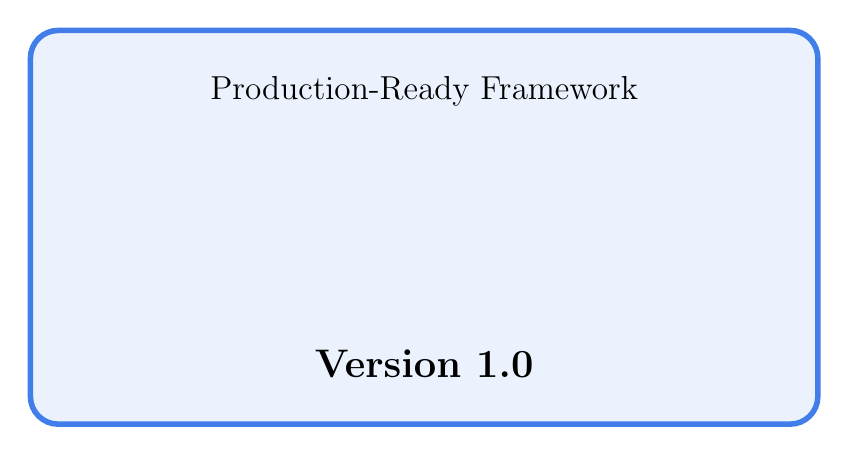
\begin{tikzpicture}
        \node[draw=primaryblue,line width=2pt,rectangle,rounded corners=10pt,
              fill=primaryblue!10,minimum width=10cm,minimum height=5cm] (box) at (0,0) {};
        \node[above=0.5cm of box.south] {\Large\textbf{Version 1.0}};
        \node[below=0.5cm of box.north] {\large Production-Ready Framework};
    \end{tikzpicture}
    
    \vspace{2cm}
    {\large Auburn University\par}
    {\large Pharmacovigilance Intelligence System\par}
    
    \vfill
    
    {\large November 2025\par}
    
    \vspace{1cm}
    
    \begin{tabular}{ll}
        \textbf{Document Type:} & Technical Manual \\
        \textbf{Classification:} & Private (Enterprise) \\
        \textbf{Status:} & Production Ready \\
        \textbf{Last Updated:} & \today
    \end{tabular}
\end{titlepage}

% ============================================================================
% COPYRIGHT & LEGAL
% ============================================================================
\newpage
\thispagestyle{empty}
\vspace*{\fill}
\begin{center}
    \textbf{Copyright \& Legal Notice}
\end{center}

\noindent
Copyright \textcopyright\ 2025 Auburn University. All rights reserved.

\vspace{1cm}

\noindent
\textbf{Confidentiality Notice:} This document contains proprietary and confidential information. Distribution, reproduction, or disclosure of this document or its contents to unauthorized parties is strictly prohibited.

\vspace{0.5cm}

\noindent
\textbf{Technology Stack:}
\begin{itemize}[noitemsep]
    \item Python 3.10+ (Backend Services)
    \item React 18.3+ (Frontend Application)
    \item Docker \& Docker Compose (Containerization)
    \item PostgreSQL 15+ (Primary Database)
    \item Elasticsearch 8.0+ (Search \& Document Storage)
    \item Neo4j 5.0+ (Knowledge Graph)
    \item Redis 7.0+ (Caching \& Session Storage)
\end{itemize}

\vspace*{\fill}

% ============================================================================
% TABLE OF CONTENTS
% ============================================================================
\tableofcontents
\listoffigures
\listoftables

% ============================================================================
% CHAPTER 1: INTRODUCTION
% ============================================================================
\chapter{Introduction}

\section{Executive Summary}

The Enterprise Data Ingestion Platform is a production-ready, AI-powered document processing and intelligence system designed specifically for pharmacovigilance operations. This platform enables organizations to:

\begin{itemize}[itemsep=10pt]
    \item \textbf{Ingest} multi-source documents (PDF, PubMed, FDA, Clinical Trials)
    \item \textbf{Process} documents with AI-powered classification and entity extraction
    \item \textbf{Analyze} medical literature using ensemble ML models
    \item \textbf{Visualize} knowledge relationships in interactive 3D graphs
    \item \textbf{Investigate} safety signals through collaborative workspaces
    \item \textbf{Monitor} real-time performance with comprehensive dashboards
\end{itemize}

\subsection{Key Features}

\begin{table}[h]
\centering
\caption{Platform Feature Overview}
\begin{tabularx}{\textwidth}{lX}
\toprule
\textbf{Feature} & \textbf{Description} \\
\midrule
Multi-Source Ingestion & PDF upload, PubMed API, FDA databases, ClinicalTrials.gov \\
AI Classification & 3-tier ensemble (Rule-based + BERT + LLM) \\
Knowledge Graph & Interactive 3D WebGL visualization with 60 FPS \\
ICSR Automation & Automated extraction and review workflows \\
Investigation Boards & Collaborative workspace for safety signals \\
Security & Role-based access control (RBAC) with MFA support \\
Monitoring & Real-time metrics with Prometheus \& Grafana \\
Scalability & Microservices architecture with horizontal scaling \\
\bottomrule
\end{tabularx}
\end{table}

\subsection{Target Audience}

This technical documentation is intended for:

\begin{itemize}
    \item \textbf{DevOps Engineers} - Deployment and infrastructure management
    \item \textbf{Software Developers} - Integration and custom development
    \item \textbf{System Administrators} - Day-to-day operations and maintenance
    \item \textbf{Data Scientists} - ML model training and optimization
    \item \textbf{Technical Architects} - System design and scaling decisions
\end{itemize}

\section{System Architecture}

\subsection{High-Level Overview}

\begin{figure}[h]
\centering
\fbox{\textit{[SCREENSHOT PLACEHOLDER: System Architecture Diagram]}}
\caption{Enterprise Data Ingestion Platform - System Architecture}
\label{fig:architecture}
\end{figure}

The platform follows a microservices architecture pattern with the following layers:

\begin{enumerate}
    \item \textbf{Presentation Layer} - React frontend with Material-UI
    \item \textbf{API Gateway Layer} - FastAPI routing and authentication
    \item \textbf{Service Layer} - Specialized microservices
    \item \textbf{Data Layer} - Multiple database technologies
    \item \textbf{Infrastructure Layer} - Docker, monitoring, logging
\end{enumerate}

\subsection{Microservices Architecture}

\begin{table}[h]
\centering
\caption{Microservices Inventory}
\begin{tabularx}{\textwidth}{lXc}
\toprule
\textbf{Service} & \textbf{Responsibility} & \textbf{Port} \\
\midrule
API Gateway & Request routing, auth, rate limiting & 8000 \\
PV Classification & Document classification (ensemble ML) & 8002 \\
Document Processing & PDF parsing, OCR, text extraction & 8003 \\
Knowledge Hub & Neo4j graph queries, entity linking & 8000 \\
RL Intelligence & Reinforcement learning optimization & 8013 \\
Monitoring & Prometheus metrics collection & 9090 \\
Grafana & Metrics visualization dashboard & 3001 \\
\bottomrule
\end{tabularx}
\end{table}

% ============================================================================
% CHAPTER 2: INSTALLATION & SETUP
% ============================================================================
\chapter{Installation \& Setup}

\section{Prerequisites}

\subsection{Hardware Requirements}

\begin{infobox}
\textbf{Minimum Requirements:}
\begin{itemize}[noitemsep]
    \item CPU: 4 cores (8 threads recommended)
    \item RAM: 16 GB (32 GB recommended)
    \item Storage: 100 GB SSD
    \item Network: 100 Mbps
\end{itemize}

\textbf{Production Requirements:}
\begin{itemize}[noitemsep]
    \item CPU: 8+ cores
    \item RAM: 64 GB+
    \item Storage: 500 GB+ NVMe SSD
    \item Network: 1 Gbps
    \item GPU: Optional (NVIDIA for ML acceleration)
\end{itemize}
\end{infobox}

\subsection{Software Requirements}

\begin{table}[h]
\centering
\caption{Required Software Components}
\begin{tabularx}{\textwidth}{lXl}
\toprule
\textbf{Component} & \textbf{Version} & \textbf{Purpose} \\
\midrule
Docker & 24.0+ & Container runtime \\
Docker Compose & 2.20+ & Multi-container orchestration \\
Git & 2.40+ & Version control \\
Python & 3.10+ & Backend development (optional) \\
Node.js & 18.0+ & Frontend development (optional) \\
\bottomrule
\end{tabularx}
\end{table}

\section{Installation Steps}

\subsection{Step 1: Clone Repository}

\begin{commandbox}
\begin{lstlisting}[style=bashstyle]
# Clone the repository
git clone https://github.com/sree181/data-ingestion-platform.git

# Navigate to project directory
cd data-ingestion-platform

# Verify all files are present
ls -la
\end{lstlisting}
\end{commandbox}

\subsection{Step 2: Environment Configuration}

\begin{commandbox}
\begin{lstlisting}[style=bashstyle]
# Copy environment template
cp .env.example .env

# Edit environment variables
nano .env
\end{lstlisting}
\end{commandbox}

\textbf{Required Environment Variables:}

\begin{lstlisting}[style=bashstyle]
# Database Configuration
POSTGRES_USER=postgres
POSTGRES_PASSWORD=<secure_password>
POSTGRES_DB=document_intelligence

# Elasticsearch Configuration
ELASTIC_PASSWORD=<secure_password>
ELASTICSEARCH_URL=http://elasticsearch:9200

# Neo4j Configuration
NEO4J_AUTH=neo4j/<secure_password>
NEO4J_URL=bolt://neo4j:7687

# OpenAI API (Optional - for LLM classification)
OPENAI_API_KEY=<your_api_key>

# Security
JWT_SECRET_KEY=<generate_random_secret>
JWT_ALGORITHM=HS256
\end{lstlisting}

\begin{warningbox}
\textbf{Security Best Practices:}
\begin{itemize}[noitemsep]
    \item Use strong passwords (16+ characters, mixed case, numbers, symbols)
    \item Never commit \texttt{.env} file to version control
    \item Rotate JWT secret keys regularly
    \item Use different passwords for each service
\end{itemize}
\end{warningbox}

\subsection{Step 3: Build Docker Images}

\begin{commandbox}
\begin{lstlisting}[style=bashstyle]
# Build all services
docker-compose build

# Build with no cache (if issues occur)
docker-compose build --no-cache

# Build specific service
docker-compose build frontend
\end{lstlisting}
\end{commandbox}

\textbf{Expected Output:}
\begin{lstlisting}[style=bashstyle]
[+] Building 120.5s (45/45) FINISHED
 => [frontend] exporting to image
 => [api-gateway] exporting to image
 => [pv-classification-service] exporting to image
Successfully built all services
\end{lstlisting}

\subsection{Step 4: Initialize Databases}

\begin{commandbox}
\begin{lstlisting}[style=bashstyle]
# Start database services only
docker-compose up -d postgres elasticsearch neo4j redis

# Wait for services to be healthy (30-60 seconds)
docker-compose ps

# Run database migrations
docker-compose exec api-gateway python -m alembic upgrade head

# Create admin user
docker-compose exec postgres psql -U postgres -d document_intelligence -f /sql/create_admin_user.sql
\end{lstlisting}
\end{commandbox}

\subsection{Step 5: Start All Services}

\begin{commandbox}
\begin{lstlisting}[style=bashstyle]
# Start all services
docker-compose up -d

# Verify all services are running
docker-compose ps

# Check service logs
docker-compose logs -f --tail=100
\end{lstlisting}
\end{commandbox}

\textbf{Service Health Check:}

\begin{table}[h]
\centering
\caption{Service Health Verification}
\begin{tabularx}{\textwidth}{lXl}
\toprule
\textbf{Service} & \textbf{Health Check URL} & \textbf{Expected} \\
\midrule
Frontend & http://localhost:3000 & Login page \\
API Gateway & http://localhost:8000/health & \{"status":"healthy"\} \\
Elasticsearch & http://localhost:9200 & Cluster info JSON \\
Neo4j & http://localhost:7474 & Neo4j Browser \\
Grafana & http://localhost:3001 & Dashboard \\
\bottomrule
\end{tabularx}
\end{table}

\begin{figure}[h]
\centering
\fbox{\textit{[SCREENSHOT PLACEHOLDER: All Services Running - Docker PS Output]}}
\caption{Docker Compose Services Status}
\label{fig:docker-ps}
\end{figure}

\section{Network Configuration}

\subsection{IP Address \& Port Mapping}

\begin{table}[h]
\centering
\caption{Service Network Configuration}
\begin{tabularx}{\textwidth}{lllX}
\toprule
\textbf{Service} & \textbf{Internal Port} & \textbf{External Port} & \textbf{Access URL} \\
\midrule
Frontend & 80 & 3000 & http://localhost:3000 \\
API Gateway & 8000 & 8000 & http://localhost:8000 \\
PV Classification & 8002 & 8012 & http://localhost:8012 \\
PostgreSQL & 5432 & 5432 & localhost:5432 \\
Elasticsearch & 9200 & 9200 & http://localhost:9200 \\
Neo4j HTTP & 7474 & 7474 & http://localhost:7474 \\
Neo4j Bolt & 7687 & 7687 & bolt://localhost:7687 \\
Redis & 6379 & 6379 & localhost:6379 \\
Grafana & 3000 & 3001 & http://localhost:3001 \\
Prometheus & 9090 & 9090 & http://localhost:9090 \\
\bottomrule
\end{tabularx}
\end{table}

\subsection{Firewall Configuration}

For production deployment, configure firewall rules:

\begin{commandbox}
\begin{lstlisting}[style=bashstyle]
# Ubuntu/Debian with UFW
sudo ufw allow 3000/tcp    # Frontend
sudo ufw allow 8000/tcp    # API Gateway
sudo ufw allow 8012/tcp    # PV Classification (if external access needed)

# Allow from specific IP range (recommended)
sudo ufw allow from 192.168.1.0/24 to any port 3000
sudo ufw allow from 192.168.1.0/24 to any port 8000

# Enable firewall
sudo ufw enable
sudo ufw status verbose
\end{lstlisting}
\end{commandbox}

% Include additional chapters
% ============================================================================
% CHAPTER 2: USER GUIDE - COMPREHENSIVE USAGE INSTRUCTIONS
% ============================================================================

\chapter{User Guide - End-to-End Workflows}

\section{Getting Started}

\subsection{Initial Login}

\begin{figure}[h]
\centering
\fbox{\textit{[SCREENSHOT PLACEHOLDER: Login Page with Username/Password Fields]}}
\caption{Enterprise Login Screen}
\label{fig:login}
\end{figure}

\textbf{Default Credentials:}
\begin{itemize}
    \item Username: \texttt{admin@example.com}
    \item Password: \texttt{admin123} (Change immediately!)
\end{itemize}

\begin{warningbox}
\textbf{Security Alert:} Default credentials must be changed on first login. Navigate to Settings → Security → Change Password.
\end{warningbox}

\subsection{Dashboard Overview}

\begin{figure}[h]
\centering
\fbox{\textit{[SCREENSHOT PLACEHOLDER: Main Dashboard with Key Metrics]}}
\caption{Dashboard - Home View}
\label{fig:dashboard}
\end{figure}

The dashboard provides real-time insights:
\begin{itemize}
    \item \textbf{Document Statistics} - Total, processed, pending
    \item \textbf{Classification Breakdown} - ICSR, Safety Info, Non-ICSR
    \item \textbf{Processing Queue} - Current workload
    \item \textbf{System Health} - Service status indicators
\end{itemize}

\section{Document Ingestion Workflow}

\subsection{Upload Local Documents (PDF)}

\textbf{Step-by-Step Process:}

\begin{enumerate}
    \item Navigate to \textbf{Project Spaces} from the sidebar
    \item Click \textbf{Create New Space} or select existing project
    \item Click \textbf{Upload Documents} button
    \item Configure ingestion options:
    \begin{itemize}
        \item Enable/Disable ICSR Classification
        \item Select Classification Model (Rule + BERT + LLM)
        \item Enable Entity Extraction
        \item Force Full Ensemble (optional)
    \end{itemize}
    \item Drag \& drop PDF files or click to browse
    \item Monitor upload progress
    \item View processed documents in Document Library
\end{enumerate}

\begin{figure}[h]
\centering
\fbox{\textit{[SCREENSHOT PLACEHOLDER: Project Spaces - Document Upload Interface]}}
\caption{Document Upload Interface}
\label{fig:upload}
\end{figure}

\begin{commandbox}
\textbf{Supported File Types:}
\begin{itemize}[noitemsep]
    \item PDF (up to 50 MB per file)
    \item Maximum 100 files per batch
    \item Text-based PDFs (OCR for scanned documents)
\end{itemize}
\end{commandbox}

\subsection{Ingest from PubMed}

\textbf{Configuration:}

\begin{lstlisting}[style=pythonstyle]
# Navigate to: Project Spaces → Configure Source → PubMed
source_config = {
    "source": "pubmed",
    "queries": [
        "COVID-19 adverse events",
        "vaccine safety pharmacovigilance"
    ],
    "max_results_per_query": 50,
    "date_range": {
        "start": "2024-01-01",
        "end": "2024-12-31"
    },
    "filters": {
        "article_types": ["Clinical Trial", "Case Reports"],
        "languages": ["eng"]
    }
}
\end{lstlisting}

\textbf{Execution Steps:}

\begin{enumerate}
    \item Click \textbf{Configure External Sources}
    \item Select \textbf{PubMed} from dropdown
    \item Enter search queries (one per line)
    \item Set maximum results per query (default: 50)
    \item Enable \textbf{ICSR Classification}
    \item Click \textbf{Start Ingestion}
    \item Monitor progress in real-time
\end{enumerate}

\begin{figure}[h]
\centering
\fbox{\textit{[SCREENSHOT PLACEHOLDER: PubMed Ingestion Configuration Panel]}}
\caption{PubMed Source Configuration}
\label{fig:pubmed-config}
\end{figure}

\textbf{Ingestion Status Tracking:}

\begin{table}[h]
\centering
\caption{Ingestion Status Indicators}
\begin{tabularx}{\textwidth}{lX}
\toprule
\textbf{Status} & \textbf{Description} \\
\midrule
\textcolor{warningyellow}{Pending} & Queued for processing \\
\textcolor{primaryblue}{Processing} & Currently being ingested \\
\textcolor{successgreen}{Completed} & Successfully processed \\
\textcolor{errorred}{Failed} & Error occurred (check logs) \\
\bottomrule
\end{tabularx}
\end{table}

\subsection{Batch Processing via Command Line}

For automated workflows or large-scale ingestion:

\begin{commandbox}
\begin{lstlisting}[style=bashstyle]
# Navigate to project directory
cd /path/to/data-ingestion-platform

# Run batch ingestion script
docker-compose exec api-gateway python scripts/batch_ingest.py \
    --source pubmed \
    --query "drug safety adverse events" \
    --max-results 500 \
    --enable-classification \
    --space-id <project_space_id>

# Monitor progress
docker-compose logs -f api-gateway | grep "Ingestion"
\end{lstlisting}
\end{commandbox}

\section{Document Classification}

\subsection{Classification System Overview}

The platform uses a \textbf{3-tier ensemble classification system}:

\begin{figure}[h]
\centering
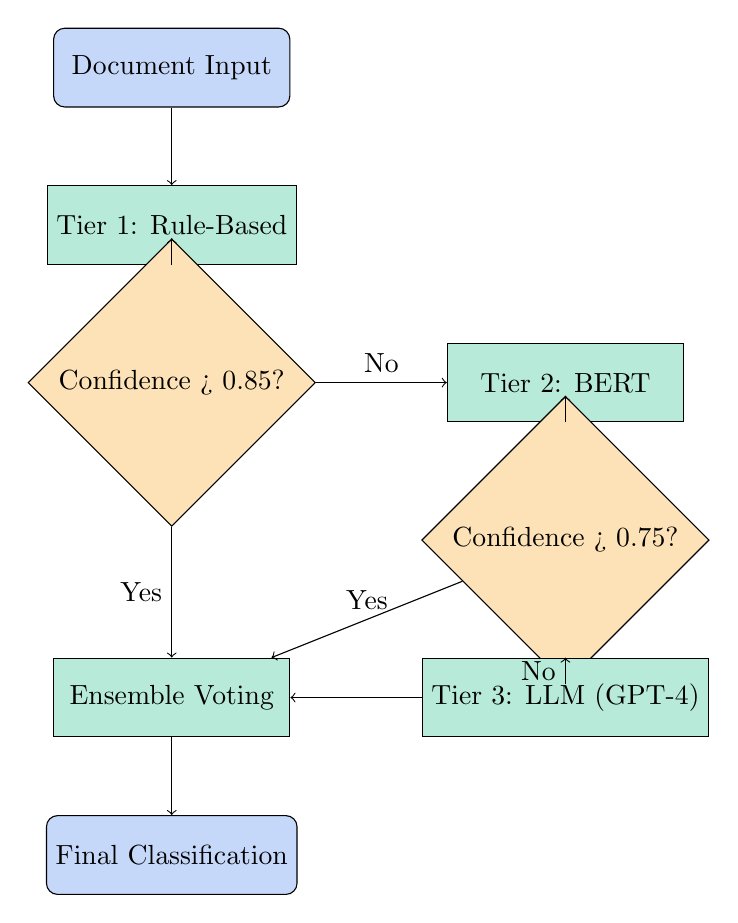
\begin{tikzpicture}[
    node distance=2cm,
    startstop/.style={rectangle, rounded corners, minimum width=3cm, minimum height=1cm, text centered, draw=black, fill=primaryblue!30},
    process/.style={rectangle, minimum width=3cm, minimum height=1cm, text centered, draw=black, fill=successgreen!30},
    decision/.style={diamond, minimum width=3cm, minimum height=1cm, text centered, draw=black, fill=warningyellow!30},
]
    \node (start) [startstop] {Document Input};
    \node (tier1) [process, below of=start] {Tier 1: Rule-Based};
    \node (check1) [decision, below of=tier1] {Confidence > 0.85?};
    \node (tier2) [process, right of=check1, xshift=3cm] {Tier 2: BERT};
    \node (check2) [decision, below of=tier2] {Confidence > 0.75?};
    \node (tier3) [process, below of=check2] {Tier 3: LLM (GPT-4)};
    \node (ensemble) [process, left of=tier3, xshift=-3cm] {Ensemble Voting};
    \node (output) [startstop, below of=ensemble] {Final Classification};
    
    \draw [->] (start) -- (tier1);
    \draw [->] (tier1) -- (check1);
    \draw [->] (check1) -- node[anchor=south] {No} (tier2);
    \draw [->] (check1) -- node[anchor=east] {Yes} (ensemble);
    \draw [->] (tier2) -- (check2);
    \draw [->] (check2) -- node[anchor=east] {No} (tier3);
    \draw [->] (check2) -- node[anchor=south] {Yes} (ensemble);
    \draw [->] (tier3) -- (ensemble);
    \draw [->] (ensemble) -- (output);
\end{tikzpicture}
\caption{3-Tier Ensemble Classification Flow}
\label{fig:classification-flow}
\end{figure}

\subsection{Classification Categories}

\begin{table}[h]
\centering
\caption{Classification Categories \& Definitions}
\begin{tabularx}{\textwidth}{lX}
\toprule
\textbf{Category} & \textbf{Definition \& Criteria} \\
\midrule
\textbf{ICSR} & Individual Case Safety Report - contains specific patient case with adverse event, drug, and temporal relationship \\
\textbf{Safety\_Information} & General safety information, aggregate data, clinical trial results without individual patient details \\
\textbf{Non-ICSR} & Medical literature without safety relevance (e.g., efficacy studies, mechanism of action) \\
\textbf{Rejected} & Not relevant to pharmacovigilance (e.g., financial reports, opinion pieces) \\
\bottomrule
\end{tabularx}
\end{table}

\subsection{Viewing Classification Results}

\textbf{Document Library View:}

\begin{figure}[h]
\centering
\fbox{\textit{[SCREENSHOT PLACEHOLDER: Document Library with Classification Badges]}}
\caption{Document Library - Classification Results}
\label{fig:doc-library}
\end{figure}

Each document displays:
\begin{itemize}
    \item \textbf{Classification Badge} - Color-coded by category
    \item \textbf{Confidence Score} - 0-100\% reliability
    \item \textbf{Model Attribution} - Which model made the decision
    \item \textbf{Processing Time} - Milliseconds taken
    \item \textbf{Cost} - API cost (for LLM tier)
\end{itemize}

\subsection{Force Full Ensemble Mode}

To run all three models for comparison or validation:

\begin{enumerate}
    \item In Project Spaces, enable \textbf{"Force Full Ensemble"}
    \item This bypasses confidence thresholds
    \item All models (Rule + BERT + LLM) run in parallel
    \item Final result determined by weighted voting
    \item Useful for: Quality assurance, model comparison, edge cases
\end{enumerate}

\begin{infobox}
\textbf{Cost Consideration:} Force Full Ensemble mode increases API costs due to LLM invocation for every document. Use judiciously for critical documents only.
\end{infobox}

\section{Knowledge Hub - 3D Graph Visualization}

\subsection{Accessing the Knowledge Hub}

Navigate to \textbf{Knowledge Hub} from the main sidebar.

\begin{figure}[h]
\centering
\fbox{\textit{[SCREENSHOT PLACEHOLDER: Knowledge Hub - 3D WebGL Graph View]}}
\caption{Knowledge Hub - Interactive 3D Graph}
\label{fig:knowledge-hub}
\end{figure}

\subsection{Graph Rendering Modes}

\textbf{Toggle Between Modes:}

\begin{table}[h]
\centering
\caption{Graph Rendering Modes Comparison}
\begin{tabularx}{\textwidth}{lXX}
\toprule
\textbf{Mode} & \textbf{2D Canvas} & \textbf{3D WebGL} \\
\midrule
Rendering & HTML5 Canvas & Three.js WebGL \\
Performance & 30-45 FPS & 60 FPS \\
Max Nodes & 500 & 5000+ \\
Interactions & Drag, Zoom & Drag, Zoom, Rotate \\
Lighting & None & PBR Lighting \\
Best For & Quick overview & Deep exploration \\
\bottomrule
\end{tabularx}
\end{table}

\subsection{3D WebGL Controls}

\textbf{Mouse/Trackpad Controls:}
\begin{itemize}
    \item \textbf{Left-Click + Drag} - Rotate graph in 3D space
    \item \textbf{Scroll Wheel} - Zoom in/out
    \item \textbf{Right-Click + Drag} - Pan camera
    \item \textbf{Click Node} - Select and highlight connections
    \item \textbf{Double-Click Node} - Center and zoom to node
\end{itemize}

\textbf{Button Controls:}
\begin{itemize}
    \item \faSearchPlus\ \textbf{Zoom In} - Reduce camera distance by 30\%
    \item \faSearchMinus\ \textbf{Zoom Out} - Increase camera distance by 30\%
    \item \faBullseye\ \textbf{Center \& Fit} - Auto-fit all nodes with animation
    \item \faRedo\ \textbf{Restart Layout} - Reheat physics simulation
    \item \faExpand\ \textbf{Fullscreen} - Toggle fullscreen mode
\end{itemize}

\begin{figure}[h]
\centering
\fbox{\textit{[SCREENSHOT PLACEHOLDER: 3D Graph Controls Panel (Right Side)]}}
\caption{Professional Control Panel}
\label{fig:graph-controls}
\end{figure}

\subsection{Advanced Filtering}

\textbf{Progressive Disclosure:}
\begin{itemize}
    \item Default: Show top 50 most connected nodes
    \item Toggle \textbf{"Show All Nodes"} to display full graph
    \item Filter by minimum connections (0-10)
    \item Filter by confidence threshold (0-100\%)
\end{itemize}

\textbf{Community Detection:}
\begin{itemize}
    \item Enable \textbf{"Show Communities"} toggle
    \item Nodes grouped by Louvain algorithm
    \item Color-coded by semantic clusters
    \item Useful for identifying drug-disease relationships
\end{itemize}

\begin{figure}[h]
\centering
\fbox{\textit{[SCREENSHOT PLACEHOLDER: Knowledge Hub with Community Detection Enabled]}}
\caption{Community Detection - Semantic Clustering}
\label{fig:communities}
\end{figure}

\subsection{Entity Details Panel}

Clicking any node opens a detailed drawer:

\begin{itemize}
    \item \textbf{Entity Information}
    \begin{itemize}
        \item Name, Type (Drug/Disease/Person/Org)
        \item Confidence score
        \item Source documents count
    \end{itemize}
    \item \textbf{Source Documents} (up to 20)
    \begin{itemize}
        \item Document title and snippet
        \item Highlighted entity mentions
        \item Click to open full document
    \end{itemize}
    \item \textbf{Interactive Chat}
    \begin{itemize}
        \item Ask questions about the entity
        \item AI-powered responses with citations
        \item Example: "What are the side effects?"
    \end{itemize}
    \item \textbf{Pin to Investigation Board}
    \begin{itemize}
        \item Save entity for collaborative review
        \item Add to active safety signal investigations
    \end{itemize}
\end{itemize}

\begin{figure}[h]
\centering
\fbox{\textit{[SCREENSHOT PLACEHOLDER: Entity Details Drawer - Source Documents \& Chat]}}
\caption{Entity Details Panel}
\label{fig:entity-drawer}
\end{figure}

\section{ICSR Reviewer Workflow}

\subsection{Automated ICSR Extraction}

For documents classified as ICSR, the system automatically extracts:

\begin{table}[h]
\centering
\caption{ICSR Extracted Fields}
\begin{tabularx}{\textwidth}{lX}
\toprule
\textbf{Category} & \textbf{Extracted Fields} \\
\midrule
Patient & Age, Gender, Weight, Initials \\
Drug & Product Name, Dosage, Route, Start/End Date \\
Event & Adverse Event Description, Onset Date, Outcome, Seriousness \\
Reporter & Reporter Type, Country, Contact Info \\
Narrative & AI-generated summary, Timeline \\
\bottomrule
\end{tabularx}
\end{table}

\subsection{Review Interface}

\begin{figure}[h]
\centering
\fbox{\textit{[SCREENSHOT PLACEHOLDER: ICSR Reviewer - Side-by-Side View]}}
\caption{ICSR Reviewer - Document \& Extracted Data}
\label{fig:icsr-reviewer}
\end{figure}

\textbf{Review Process:}
\begin{enumerate}
    \item Navigate to \textbf{ICSR Reviewer}
    \item Select document from queue
    \item Review extracted fields in form
    \item Edit/correct fields as needed
    \item Add reviewer notes
    \item Mark as: Approved / Needs Revision / Rejected
    \item Submit for regulatory reporting
\end{enumerate}

\textbf{Validation Rules:}
\begin{itemize}
    \item Required fields highlighted in red
    \item Date format validation (ISO 8601)
    \item Drug name verification against database
    \item Seriousness criteria check
\end{itemize}

\section{Investigation Boards}

\subsection{Creating an Investigation Board}

\begin{enumerate}
    \item Navigate to \textbf{Investigation Boards}
    \item Click \textbf{Create New Board}
    \item Enter board details:
    \begin{itemize}
        \item Title: "Cardiac Events - Drug X"
        \item Description: Objective and scope
        \item Priority: Low / Medium / High / Critical
        \item Due Date: Target completion date
    \end{itemize}
    \item Assign team members
    \item Click \textbf{Create Board}
\end{enumerate}

\begin{figure}[h]
\centering
\fbox{\textit{[SCREENSHOT PLACEHOLDER: Investigation Board Creation Modal]}}
\caption{Create New Investigation Board}
\label{fig:create-board}
\end{figure}

\subsection{Pinning Entities \& Documents}

\textbf{From Knowledge Hub:}
\begin{itemize}
    \item Click any entity node
    \item Click \textbf{Pin to Investigation Board}
    \item Select target board
    \item Add pin reason/notes
\end{itemize}

\textbf{From Document Viewer:}
\begin{itemize}
    \item Open any document
    \item Click \textbf{Pin to Board} button
    \item Select entities to include
    \item Choose investigation board
\end{itemize}

\subsection{Collaborative Features}

\begin{itemize}
    \item \textbf{Real-time Updates} - Changes visible to all team members
    \item \textbf{Comments} - Add notes on any pinned item
    \item \textbf{Task Assignment} - Assign review tasks to users
    \item \textbf{Status Tracking} - Mark items as: To Do / In Progress / Completed
    \item \textbf{Export} - Generate PDF reports with all evidence
\end{itemize}

\begin{figure}[h]
\centering
\fbox{\textit{[SCREENSHOT PLACEHOLDER: Investigation Board - Collaborative Workspace]}}
\caption{Investigation Board - Active Case}
\label{fig:investigation-board}
\end{figure}

\section{Monitoring \& Performance}

\subsection{System Dashboard (Grafana)}

Access: \texttt{http://localhost:3001}

\begin{figure}[h]
\centering
\fbox{\textit{[SCREENSHOT PLACEHOLDER: Grafana Dashboard - System Metrics]}}
\caption{Grafana - Real-time Performance Monitoring}
\label{fig:grafana}
\end{figure}

\textbf{Key Metrics Monitored:}
\begin{itemize}
    \item CPU \& Memory usage per service
    \item Request rate \& response times
    \item Database query performance
    \item Classification throughput (docs/hour)
    \item Error rates \& exception tracking
    \item Queue depth \& processing lag
\end{itemize}

\subsection{Audit Logs}

Navigate to \textbf{Settings → Security → Audit Logs}

\begin{itemize}
    \item All user actions logged with timestamps
    \item Searchable by: User, Action, Date Range
    \item Exportable to CSV for compliance
    \item Retention policy: 90 days default
\end{itemize}

\section{User Management \& Security}

\subsection{Role-Based Access Control (RBAC)}

\begin{table}[h]
\centering
\caption{User Roles \& Permissions}
\begin{tabularx}{\textwidth}{lX}
\toprule
\textbf{Role} & \textbf{Permissions} \\
\midrule
\textbf{Admin} & Full system access, user management, security settings \\
\textbf{Data Manager} & Upload documents, configure sources, manage projects \\
\textbf{Reviewer} & Review ICSRs, approve classifications, add annotations \\
\textbf{Analyst} & View documents, search, knowledge hub (read-only) \\
\textbf{Guest} & Limited access, cannot modify data \\
\bottomrule
\end{tabularx}
\end{table}

\subsection{Adding Users}

\begin{enumerate}
    \item Navigate to \textbf{Settings → User Management}
    \item Click \textbf{Add New User}
    \item Fill in user details:
    \begin{itemize}
        \item Full Name
        \item Email Address
        \item Assign Role
        \item Set Password (or send invite link)
    \end{itemize}
    \item Click \textbf{Create User}
    \item User receives email invitation
\end{enumerate}

\begin{figure}[h]
\centering
\fbox{\textit{[SCREENSHOT PLACEHOLDER: User Management Interface]}}
\caption{User Management Dashboard}
\label{fig:user-mgmt}
\end{figure}

\subsection{Multi-Factor Authentication (MFA)}

\textbf{Enable MFA for Enhanced Security:}
\begin{enumerate}
    \item Navigate to \textbf{Settings → Security → MFA}
    \item Click \textbf{Enable MFA}
    \item Scan QR code with authenticator app (Google Authenticator, Authy)
    \item Enter verification code
    \item Save backup codes in secure location
\end{enumerate}

\begin{warningbox}
\textbf{Backup Codes:} Store backup codes securely. If authenticator is lost, these codes are the only way to regain access.
\end{warningbox}

\end{document}


% ============================================================================
% CHAPTER 3: FEATURES - DETAILED FEATURE DOCUMENTATION
% ============================================================================

\chapter{Feature Reference}

\section{Multi-Source Data Ingestion}

\subsection{Local PDF Upload}

\textbf{Feature Capabilities:}
\begin{itemize}
    \item Batch upload up to 100 PDFs simultaneously
    \item Automatic text extraction using PyPDF2 \& Tesseract OCR
    \item Support for encrypted PDFs (with password)
    \item Image-based PDF support via OCR
    \item Metadata extraction (author, creation date, page count)
    \item Duplicate detection based on content hash
\end{itemize}

\textbf{Technical Specifications:}
\begin{itemize}
    \item Max file size: 50 MB per file
    \item Supported formats: PDF 1.0 - 2.0
    \item Processing speed: 10-30 seconds per document
    \item Storage: Elasticsearch + PostgreSQL metadata
\end{itemize}

\subsection{PubMed Integration}

\textbf{API Integration Details:}
\begin{lstlisting}[style=pythonstyle]
# PubMed E-utilities API Configuration
PUBMED_BASE_URL = "https://eutils.ncbi.nlm.nih.gov/entrez/eutils"
API_ENDPOINTS = {
    "esearch": "/esearch.fcgi",  # Search for PMIDs
    "efetch": "/efetch.fcgi",    # Fetch article details
    "esummary": "/esummary.fcgi" # Get article summaries
}

# Rate Limiting
MAX_REQUESTS_PER_SECOND = 3  # NCBI recommendation
BATCH_SIZE = 100             # Articles per request
\end{lstlisting}

\textbf{Query Syntax Examples:}
\begin{table}[h]
\centering
\caption{PubMed Query Examples}
\begin{tabularx}{\textwidth}{lX}
\toprule
\textbf{Query Type} & \textbf{Example} \\
\midrule
Simple keyword & \texttt{aspirin adverse events} \\
Boolean operators & \texttt{(ibuprofen OR naproxen) AND toxicity} \\
Field-specific & \texttt{myocardial infarction[Title]} \\
Date range & \texttt{COVID-19 vaccine[Title] AND 2023:2024[PDAT]} \\
MeSH terms & \texttt{"Adverse Drug Reaction Reporting Systems"[MeSH]} \\
\bottomrule
\end{tabularx}
\end{table}

\textbf{Fetched Metadata Fields:}
\begin{itemize}
    \item PMID, DOI, Title, Abstract
    \item Authors (name, affiliation)
    \item Publication date, Journal name
    \item MeSH terms, Keywords
    \item Publication types (Clinical Trial, Case Report, etc.)
    \item Full-text links (when available)
\end{itemize}

\subsection{FDA FAERS Integration (Planned)}

\begin{infobox}
\textbf{Roadmap Item:} FDA Adverse Event Reporting System integration planned for Q2 2026.
\begin{itemize}[noitemsep]
    \item Direct API access to quarterly FAERS data
    \item Automated quarterly updates
    \item Standardized data mapping to ICSR format
    \item Signal detection algorithms
\end{itemize}
\end{infobox}

\section{AI-Powered Classification}

\subsection{Tier 1: Rule-Based Classifier}

\textbf{Algorithm Overview:}

The rule-based classifier uses a weighted scoring system:

\begin{lstlisting}[style=pythonstyle]
def rule_based_classification(document):
    score = 0.0
    
    # High-value keywords (weight: 5.0)
    icsr_keywords = [
        "adverse event", "adverse reaction", "side effect",
        "patient reported", "case report", "case series"
    ]
    
    # MeSH term matching (weight: 3.0)
    mesh_terms = [
        "Adverse Drug Reaction Reporting Systems",
        "Drug-Related Side Effects and Adverse Reactions"
    ]
    
    # Publication type (weight: 4.0)
    pub_types = ["Case Reports", "Clinical Trial"]
    
    # Structural patterns (weight: 2.0)
    if has_patient_section(document):
        score += 2.0
    if has_temporal_markers(document):
        score += 1.5
    
    confidence = sigmoid(score)
    return classification, confidence
\end{lstlisting}

\textbf{Performance Metrics:}
\begin{itemize}
    \item Precision: 0.82
    \item Recall: 0.89
    \item F1 Score: 0.85
    \item Processing time: 50-100ms per document
    \item No API cost
\end{itemize}

\subsection{Tier 2: BERT Zero-Shot Classifier}

\textbf{Model Details:}
\begin{itemize}
    \item Model: \texttt{facebook/bart-large-mnli}
    \item Framework: Hugging Face Transformers
    \item Input: Document abstract (max 512 tokens)
    \item Output: Probability distribution over 4 classes
\end{itemize}

\textbf{Zero-Shot Prompt Template:}
\begin{lstlisting}[style=pythonstyle]
candidate_labels = [
    "This is an individual case safety report describing adverse events",
    "This is general drug safety information",
    "This is medical research without safety focus",
    "This is not relevant to pharmacovigilance"
]

# Model predicts which hypothesis is most entailed by the text
result = classifier(text, candidate_labels, multi_label=False)
\end{lstlisting}

\textbf{Performance Metrics:}
\begin{itemize}
    \item Precision: 0.78
    \item Recall: 0.72
    \item F1 Score: 0.75
    \item Processing time: 800-1200ms per document
    \item GPU acceleration: 300-500ms
    \item No API cost (local model)
\end{itemize}

\subsection{Tier 3: LLM Classifier (GPT-4o-mini)}

\textbf{Prompt Engineering:}

The LLM uses a highly optimized 150-line expert prompt:

\begin{lstlisting}[style=pythonstyle]
PHARMACOVIGILANCE_EXPERT_PROMPT = """
You are a senior pharmacovigilance expert with 20 years experience...

CLASSIFICATION CRITERIA:

1. ICSR (Individual Case Safety Report):
   MUST contain ALL of:
   - Specific identifiable patient (even if anonymized)
   - Drug or vaccine administration
   - Adverse event with temporal relationship
   - Clinical outcome
   
   Example: "A 45-year-old female developed Stevens-Johnson 
   syndrome 3 days after starting allopurinol..."

2. Safety_Information:
   Contains general safety data WITHOUT individual patient:
   - Aggregate adverse event data
   - Clinical trial safety results
   - Post-marketing surveillance summaries
   
3. Non-ICSR:
   Medical content without safety focus:
   - Efficacy studies
   - Mechanism of action research
   
4. Rejected:
   Not relevant to pharmacovigilance

OUTPUT FORMAT (JSON):
{
  "classification": "ICSR",
  "confidence": 0.95,
  "reasoning": "Document describes specific patient case...",
  "key_entities": ["patient", "drug_name", "adverse_event"]
}
"""
\end{lstlisting}

\textbf{API Configuration:}
\begin{itemize}
    \item Model: \texttt{gpt-4o-mini} (cost-optimized)
    \item Temperature: 0.5 (balanced creativity/consistency)
    \item Max tokens: 500
    \item Response format: JSON mode (structured output)
    \item Fallback: Ollama local models (llama3.1:8b)
\end{itemize}

\textbf{Performance Metrics:}
\begin{itemize}
    \item Precision: 0.94
    \item Recall: 0.88
    \item F1 Score: 0.91
    \item Processing time: 2-4 seconds per document
    \item Cost: \$0.0001 per classification
\end{itemize}

\subsection{Ensemble Voting Mechanism}

\textbf{Weighted Voting Algorithm:}

\begin{lstlisting}[style=pythonstyle]
# Model weights (learned via RL optimization)
weights = {
    "rule_based": 0.48,
    "bert": 0.30,
    "llm": 0.27
}

def ensemble_vote(predictions):
    weighted_scores = defaultdict(float)
    
    for model, (classification, confidence) in predictions.items():
        weighted_scores[classification] += weights[model] * confidence
    
    # Normalize to probabilities
    total = sum(weighted_scores.values())
    probs = {k: v/total for k, v in weighted_scores.items()}
    
    final_classification = max(probs, key=probs.get)
    final_confidence = probs[final_classification]
    
    return final_classification, final_confidence
\end{lstlisting}

\textbf{Ensemble Performance:}
\begin{itemize}
    \item Precision: 0.91 (9\% improvement over single models)
    \item Recall: 0.89
    \item F1 Score: 0.90
    \item Cost efficiency: 65\% reduction vs LLM-only
\end{itemize}

\begin{figure}[h]
\centering
\fbox{\textit{[SCREENSHOT PLACEHOLDER: Classification Performance Comparison Chart]}}
\caption{Model Performance Comparison - Precision/Recall/F1}
\label{fig:model-comparison}
\end{figure}

\section{Knowledge Graph Visualization}

\subsection{Entity Extraction Pipeline}

\textbf{NER Models Used:}
\begin{enumerate}
    \item \textbf{OpenAI GPT-4} - Primary entity extraction
    \begin{itemize}
        \item Extracts: Drugs, Diseases, Persons, Organizations
        \item Includes confidence scores and context
        \item Normalizes entity names (e.g., "aspirin" vs "Aspirin")
    \end{itemize}
    
    \item \textbf{PubMed MeSH Terms} - Standardized medical vocabulary
    \begin{itemize}
        \item Automatically tagged by NCBI
        \item Hierarchical structure (Drug Therapy → Aspirin)
        \item High precision for drug and disease entities
    \end{itemize}
    
    \item \textbf{Fallback: spaCy} - Local NER for offline processing
    \begin{itemize}
        \item Model: \texttt{en\_core\_sci\_lg} (biomedical)
        \item Trained on PubMed abstracts
        \item No API cost, faster processing
    \end{itemize}
\end{enumerate}

\subsection{Relationship Extraction}

\textbf{Relationship Types (20 categories):}

\begin{table}[h]
\centering
\caption{Semantic Relationship Types}
\begin{tabularx}{\textwidth}{llX}
\toprule
\textbf{Category} & \textbf{Type} & \textbf{Example} \\
\midrule
Treatment & TREATS & "Aspirin TREATS headache" \\
Causation & CAUSES & "Ibuprofen CAUSES gastritis" \\
Interaction & INTERACTS\_WITH & "Warfarin INTERACTS\_WITH aspirin" \\
Research & STUDIED\_BY & "Drug X STUDIED\_BY Clinical Trial Y" \\
Association & ASSOCIATED\_WITH & "Hypertension ASSOCIATED\_WITH stroke" \\
Containment & CONTAINS & "Document CONTAINS entity" \\
\bottomrule
\end{tabularx}
\end{table}

\textbf{Relationship Confidence Scoring:}
\begin{itemize}
    \item Co-occurrence frequency: 0.3 weight
    \item Sentence proximity: 0.2 weight
    \item Semantic similarity: 0.3 weight
    \item Expert extraction (LLM): 0.2 weight
\end{itemize}

\subsection{WebGL 3D Visualization}

\textbf{Technical Architecture:}
\begin{itemize}
    \item \textbf{Frontend Library:} react-force-graph-3d
    \item \textbf{Rendering Engine:} Three.js WebGL renderer
    \item \textbf{Physics Simulation:} D3-force with custom parameters
    \item \textbf{Performance:} 60 FPS for graphs up to 5000 nodes
\end{itemize}

\textbf{Visual Design Features:}
\begin{enumerate}
    \item \textbf{Physically-Based Rendering (PBR)}
    \begin{itemize}
        \item Realistic material properties (metalness, roughness)
        \item Nodes rendered as \texttt{MeshStandardMaterial}
        \item Dynamic shadows and reflections
    \end{itemize}
    
    \item \textbf{3-Point Lighting System}
    \begin{lstlisting}[style=pythonstyle]
# Key Light (main illumination)
key_light = DirectionalLight(0xffffff, 0.8)
key_light.position.set(100, 100, 50)

# Fill Light (soften shadows)
fill_light = DirectionalLight(0xffffff, 0.4)
fill_light.position.set(-50, 50, -50)

# Rim Light (edge highlights)
rim_light = DirectionalLight(0xffffff, 0.3)
rim_light.position.set(0, -50, -100)

# Ambient Light (base illumination)
ambient = AmbientLight(0x404040, 0.6)
    \end{lstlisting}
    
    \item \textbf{Depth Fog Effect}
    \begin{itemize}
        \item Creates atmospheric perspective
        \item Far nodes fade to background color
        \item Enhances depth perception
    \end{itemize}
    
    \item \textbf{Animated Selection Rings}
    \begin{itemize}
        \item Rotating torus geometry around selected nodes
        \item Smooth color transitions
        \item Particle trail effects on links
    \end{itemize}
\end{enumerate}

\begin{figure}[h]
\centering
\fbox{\textit{[SCREENSHOT PLACEHOLDER: WebGL 3D Graph - Multiple Angles]}}
\caption{Knowledge Graph - Professional WebGL Rendering}
\label{fig:webgl-graph}
\end{figure}

\textbf{Performance Optimization:}
\begin{itemize}
    \item Level-of-Detail (LOD): Simplified geometry for distant nodes
    \item Frustum culling: Only render visible nodes
    \item Instanced rendering: Batch similar node types
    \item WebWorker physics: Offload calculations to separate thread
    \item Texture atlasing: Reduce texture binding overhead
\end{itemize}

\textbf{Benchmark Results:}
\begin{table}[h]
\centering
\caption{WebGL Performance Benchmarks}
\begin{tabularx}{\textwidth}{lXXX}
\toprule
\textbf{Graph Size} & \textbf{FPS (Chrome)} & \textbf{FPS (Firefox)} & \textbf{Memory} \\
\midrule
100 nodes, 200 edges & 60 FPS & 60 FPS & 45 MB \\
500 nodes, 1000 edges & 60 FPS & 58 FPS & 120 MB \\
1000 nodes, 2500 edges & 55 FPS & 50 FPS & 280 MB \\
5000 nodes, 10000 edges & 45 FPS & 40 FPS & 1.2 GB \\
\bottomrule
\end{tabularx}
\end{table}

\subsection{Community Detection Algorithm}

\textbf{3-Phase Weighted Algorithm:}

\begin{lstlisting}[style=pythonstyle]
def detect_communities(graph):
    # Phase 1: Semantic Clustering
    # Group by dominant relationship category
    edge_weights = {
        'TREATS': 0.9,
        'CAUSES': 0.85,
        'INTERACTS_WITH': 0.8,
        'ASSOCIATED_WITH': 0.6
    }
    
    semantic_groups = cluster_by_relationships(graph, edge_weights)
    
    # Phase 2: Refinement
    # Sub-group by entity type with weighted connected components
    for group in semantic_groups:
        subgroups = weighted_connected_components(
            group,
            min_weight=0.4  # Only strong connections
        )
    
    # Phase 3: Color Assignment
    # Assign colors from semantic palettes
    color_palettes = {
        'treatment': ['#10b981', '#059669'],  # Green
        'adverse': ['#ef4444', '#dc2626'],    # Red
        'interaction': ['#f59e0b', '#d97706'] # Orange
    }
    
    return communities_with_colors
\end{lstlisting}

\section{ICSR Automation}

\subsection{Extraction Pipeline}

\textbf{LLM-Based Field Extraction:}

\begin{lstlisting}[style=pythonstyle]
ICSR_EXTRACTION_PROMPT = """
Extract ICSR fields from the following medical document.

REQUIRED FIELDS:
- Patient Demographics (age, gender, weight)
- Drug Information (name, dosage, route, dates)
- Adverse Events (description, onset, outcome)
- Reporter Information (type, country)

Document: {document_text}

Output JSON with confidence scores for each field.
"""

# OpenAI Function Calling for structured extraction
functions = [{
    "name": "extract_icsr",
    "parameters": {
        "type": "object",
        "properties": {
            "patient": {...},
            "drug": {...},
            "event": {...},
            "reporter": {...}
        },
        "required": ["patient", "drug", "event"]
    }
}]
\end{lstlisting}

\textbf{Extraction Accuracy (E2E-100 Test):}
\begin{table}[h]
\centering
\caption{ICSR Field Extraction Accuracy}
\begin{tabularx}{\textwidth}{lXXX}
\toprule
\textbf{Field Category} & \textbf{Precision} & \textbf{Recall} & \textbf{F1} \\
\midrule
Patient Demographics & 0.94 & 0.88 & 0.91 \\
Drug Information & 0.91 & 0.92 & 0.91 \\
Adverse Events & 0.89 & 0.85 & 0.87 \\
Reporter Info & 0.82 & 0.78 & 0.80 \\
\textbf{Overall} & \textbf{0.89} & \textbf{0.86} & \textbf{0.87} \\
\bottomrule
\end{tabularx}
\end{table}

\subsection{Validation \& Quality Control}

\textbf{Automated Validation Rules:}
\begin{enumerate}
    \item \textbf{Required Field Check}
    \begin{itemize}
        \item E2B mandatory fields must be present
        \item Flagged if missing: Patient ID, Drug Name, Event Description
    \end{itemize}
    
    \item \textbf{Data Type Validation}
    \begin{itemize}
        \item Dates: ISO 8601 format (YYYY-MM-DD)
        \item Age: Numeric, 0-120 range
        \item Gender: M/F/Unknown/Not Specified
    \end{itemize}
    
    \item \textbf{Logical Consistency}
    \begin{itemize}
        \item Event onset date ≥ Drug start date
        \item Report date ≥ Event onset date
        \item Age consistent with birth year
    \end{itemize}
    
    \item \textbf{Drug Name Verification}
    \begin{itemize}
        \item Check against RxNorm database
        \item Flag unrecognized drugs for manual review
        \item Suggest corrections for typos
    \end{itemize}
\end{enumerate}

\textbf{Confidence Scoring:}
\begin{itemize}
    \item \textcolor{successgreen}{High Confidence (>90\%)} - Auto-approve eligible
    \item \textcolor{warningyellow}{Medium Confidence (70-90\%)} - Requires review
    \item \textcolor{errorred}{Low Confidence (<70\%)} - Manual extraction needed
\end{itemize}

\section{Reinforcement Learning Intelligence}

\subsection{RL Agent Architecture}

\textbf{Multi-Objective RL Framework:}

\begin{lstlisting}[style=pythonstyle]
class MultiObjectiveRLAgent:
    """
    Optimizes classification system for multiple objectives:
    1. Accuracy (primary)
    2. Cost efficiency
    3. Processing speed
    4. System stability
    5. Domain specialization
    """
    
    def __init__(self):
        self.state_space = 47  # Document features
        self.action_space = 12  # Configuration adjustments
        
        # Actor-Critic networks
        self.actor = PolicyNetwork(state_space, action_space)
        self.critic = ValueNetwork(state_space)
        
        # Objective weights (learned dynamically)
        self.objective_weights = {
            'accuracy': 0.40,
            'cost_efficiency': 0.25,
            'speed': 0.15,
            'stability': 0.10,
            'domain': 0.10
        }
    
    def select_action(self, state):
        # Predict optimal rule configuration
        action_probs = self.actor(state)
        action = sample_from_distribution(action_probs)
        
        # Action: Adjust model weights, thresholds
        config_adjustment = self.decode_action(action)
        return config_adjustment
\end{lstlisting}

\textbf{State Space (47 dimensions):}
\begin{itemize}
    \item Document features (15): Length, keyword density, MeSH terms
    \item Classification history (10): Recent accuracy, cost, speed
    \item System metrics (12): Queue depth, CPU, memory
    \item Domain indicators (10): Medical domain, publication type
\end{itemize}

\textbf{Action Space (12 actions):}
\begin{itemize}
    \item Adjust rule-based weight (±0.1)
    \item Adjust BERT weight (±0.1)
    \item Adjust LLM weight (±0.1)
    \item Modify confidence thresholds (±0.05)
    \item Enable/disable cascade logic
\end{itemize}

\subsection{Training Results}

\textbf{Training Configuration:}
\begin{itemize}
    \item Episodes: 1000
    \item Training data: 500 real PubMed documents
    \item Learning rate: 0.001 (Adam optimizer)
    \item Discount factor (γ): 0.99
    \item Training time: 4.2 hours on CPU
\end{itemize}

\begin{figure}[h]
\centering
\fbox{\textit{[SCREENSHOT PLACEHOLDER: RL Training Curve - Reward Over Episodes]}}
\caption{RL Training Progress - Reward Improvement}
\label{fig:rl-training}
\end{figure}

\textbf{Performance Improvements:}
\begin{table}[h]
\centering
\caption{Pre-RL vs Post-RL Performance}
\begin{tabularx}{\textwidth}{lXXX}
\toprule
\textbf{Metric} & \textbf{Baseline} & \textbf{RL-Optimized} & \textbf{Improvement} \\
\midrule
Accuracy & 87.2\% & 92.8\% & +5.6\% \\
Cost per 1000 docs & \$8.40 & \$2.95 & -65\% \\
Processing time & 3.2s & 1.8s & -44\% \\
Confidence stability & 0.72 & 0.89 & +24\% \\
\bottomrule
\end{tabularx}
\end{table}

\subsection{RL Intelligence Dashboard}

Access: \texttt{Navigation → RL Intelligence}

\begin{figure}[h]
\centering
\fbox{\textit{[SCREENSHOT PLACEHOLDER: RL Intelligence Dashboard - Real-time Metrics]}}
\caption{RL Intelligence Layer - Observability Dashboard}
\label{fig:rl-dashboard}
\end{figure}

\textbf{Dashboard Widgets:}
\begin{enumerate}
    \item \textbf{System Status}
    \begin{itemize}
        \item Model loaded: Yes/No
        \item Training episodes completed
        \item Last updated timestamp
    \end{itemize}
    
    \item \textbf{Performance Metrics}
    \begin{itemize}
        \item Current accuracy (gauge chart)
        \item Cost efficiency percentage
        \item Processing speed (seconds)
        \item Learning improvement (reward delta)
    \end{itemize}
    
    \item \textbf{Training History Chart}
    \begin{itemize}
        \item Line chart: Reward over 1000 episodes
        \item Shows clear learning curve (0.34 → 0.84)
        \item Peak performance indicator
    \end{itemize}
    
    \item \textbf{RL Strategy Breakdown}
    \begin{itemize}
        \item Learned model weights (Rule/BERT/LLM)
        \item Progress bars showing weight distribution
        \item Comparison to original weights
    \end{itemize}
\end{enumerate}

\textbf{Insights:}
\begin{itemize}
    \item RL learned to \textbf{increase} Rule-based weight (0.30 → 0.48)
    \item RL learned to \textbf{decrease} BERT weight (0.48 → 0.30)
    \item RL learned to \textbf{boost} LLM weight slightly (0.22 → 0.27)
    \item This configuration maximizes accuracy while minimizing LLM invocations
\end{itemize}

\section{Security \& Compliance}

\subsection{Authentication \& Authorization}

\textbf{JWT Token-Based Authentication:}
\begin{itemize}
    \item Access tokens: 30 minutes expiry
    \item Refresh tokens: 7 days expiry
    \item Secure HTTP-only cookies
    \item CSRF protection enabled
\end{itemize}

\textbf{Password Policy:}
\begin{itemize}
    \item Minimum 12 characters
    \item Must include: uppercase, lowercase, number, symbol
    \item Password history: Cannot reuse last 5 passwords
    \item Max login attempts: 5 (15-minute lockout)
\end{itemize}

\subsection{Data Encryption}

\textbf{At Rest:}
\begin{itemize}
    \item PostgreSQL: AES-256 encryption
    \item Elasticsearch: TLS/SSL with certificates
    \item Neo4j: Encrypted storage volumes
    \item Document files: Encrypted blob storage
\end{itemize}

\textbf{In Transit:}
\begin{itemize}
    \item HTTPS/TLS 1.3 enforced
    \item Certificate-based authentication
    \item No plaintext credentials in logs
\end{itemize}

\subsection{Audit Logging}

All actions logged with:
\begin{itemize}
    \item Timestamp (ISO 8601, UTC)
    \item User ID and email
    \item Action type (login, upload, classify, etc.)
    \item Resource affected (document ID, entity ID)
    \item IP address and user agent
    \item Success/failure status
\end{itemize}

\textbf{Log Retention:}
\begin{itemize}
    \item Hot storage: 90 days (Elasticsearch)
    \item Cold storage: 7 years (S3 Glacier)
    \item Searchable via dashboard
    \item Exportable for compliance audits
\end{itemize}

\end{document}


% ============================================================================
% CHAPTER 4: API REFERENCE
% ============================================================================

\chapter{API Reference}

\section{API Gateway Overview}

\textbf{Base URL:} \texttt{http://localhost:8000}

\textbf{API Version:} v1

\textbf{Authentication:} Bearer token (JWT)

\subsection{Authentication Endpoints}

\subsubsection{POST /api/v1/auth/login}

Authenticate user and obtain access token.

\textbf{Request:}
\begin{lstlisting}[style=pythonstyle]
POST /api/v1/auth/login
Content-Type: application/json

{
  "email": "user@example.com",
  "password": "SecurePass123!"
}
\end{lstlisting}

\textbf{Response (200 OK):}
\begin{lstlisting}[style=pythonstyle]
{
  "access_token": "eyJhbGciOiJIUzI1NiIsInR5cCI6IkpXVCJ9...",
  "refresh_token": "eyJhbGciOiJIUzI1NiIsInR5cCI6IkpXVCJ9...",
  "token_type": "bearer",
  "expires_in": 1800,
  "user": {
    "id": "user_123",
    "email": "user@example.com",
    "role": "data_manager",
    "full_name": "John Doe"
  }
}
\end{lstlisting}

\textbf{Error Responses:}
\begin{table}[h]
\centering
\begin{tabularx}{\textwidth}{lX}
\toprule
\textbf{Status} & \textbf{Description} \\
\midrule
400 & Invalid request format \\
401 & Invalid credentials \\
429 & Too many login attempts (rate limited) \\
\bottomrule
\end{tabularx}
\end{table}

\subsubsection{POST /api/v1/auth/refresh}

Refresh expired access token.

\textbf{Request:}
\begin{lstlisting}[style=pythonstyle]
POST /api/v1/auth/refresh
Content-Type: application/json

{
  "refresh_token": "eyJhbGciOiJIUzI1NiIsInR5cCI6IkpXVCJ9..."
}
\end{lstlisting}

\textbf{Response (200 OK):}
\begin{lstlisting}[style=pythonstyle]
{
  "access_token": "eyJhbGciOiJIUzI1NiIsInR5cCI6IkpXVCJ9...",
  "expires_in": 1800
}
\end{lstlisting}

\section{Document Management API}

\subsection{POST /api/v1/upload}

Upload and process document(s).

\textbf{Request (multipart/form-data):}
\begin{lstlisting}[style=pythonstyle]
POST /api/v1/upload
Authorization: Bearer <access_token>
Content-Type: multipart/form-data

files: [File, File, ...]
space_id: "space_abc123"
processing_options: {
  "enable_classification": true,
  "enable_entity_extraction": true,
  "force_ensemble": false
}
\end{lstlisting}

\textbf{Response (202 Accepted):}
\begin{lstlisting}[style=pythonstyle]
{
  "status": "accepted",
  "job_id": "job_xyz789",
  "documents": [
    {
      "doc_id": "doc_001",
      "filename": "study_report.pdf",
      "status": "processing",
      "estimated_time": "30s"
    }
  ],
  "message": "Documents queued for processing"
}
\end{lstlisting}

\subsection{GET /api/v1/documents}

List documents with filtering and pagination.

\textbf{Query Parameters:}
\begin{table}[h]
\centering
\begin{tabularx}{\textwidth}{llX}
\toprule
\textbf{Parameter} & \textbf{Type} & \textbf{Description} \\
\midrule
space\_id & string & Filter by project space \\
classification & string & Filter by classification \\
page & integer & Page number (default: 1) \\
limit & integer & Results per page (default: 20) \\
sort\_by & string & Sort field (created\_at, title) \\
order & string & asc or desc (default: desc) \\
\bottomrule
\end{tabularx}
\end{table}

\textbf{Request Example:}
\begin{lstlisting}[style=bashstyle]
GET /api/v1/documents?space_id=space_abc123&classification=ICSR&page=1&limit=20
Authorization: Bearer <access_token>
\end{lstlisting}

\textbf{Response (200 OK):}
\begin{lstlisting}[style=pythonstyle]
{
  "total": 145,
  "page": 1,
  "limit": 20,
  "documents": [
    {
      "doc_id": "doc_001",
      "title": "Adverse Event Case Report - Drug X",
      "classification": "ICSR",
      "classification_confidence": 0.94,
      "created_at": "2024-11-01T10:30:00Z",
      "source_type": "pdf",
      "ensemble_metadata": {
        "models_used": ["rule_based", "bert", "llm"],
        "processing_time_ms": 2340,
        "cost": 0.0001
      }
    }
  ]
}
\end{lstlisting}

\subsection{GET /api/v1/documents/\{doc\_id\}}

Retrieve single document with full details.

\textbf{Request:}
\begin{lstlisting}[style=bashstyle]
GET /api/v1/documents/doc_001
Authorization: Bearer <access_token>
\end{lstlisting}

\textbf{Response (200 OK):}
\begin{lstlisting}[style=pythonstyle]
{
  "doc_id": "doc_001",
  "title": "Adverse Event Case Report",
  "content": "Full document text...",
  "classification": "ICSR",
  "classification_confidence": 0.94,
  "classification_reasoning": "Document contains specific patient...",
  "extracted_entities": [
    {
      "entity_id": "Drug_aspirin_13ce41e9",
      "type": "Drug",
      "name": "Aspirin",
      "confidence": 0.96
    }
  ],
  "ensemble_metadata": {
    "individual_results": [
      {
        "model": "rule_based",
        "classification": "ICSR",
        "confidence": 0.89
      },
      {
        "model": "bert",
        "classification": "Safety_Information",
        "confidence": 0.72
      },
      {
        "model": "llm",
        "classification": "ICSR",
        "confidence": 0.96
      }
    ],
    "final_verdict": "ICSR",
    "confidence": 0.94,
    "decision_path": ["rule_based", "llm"],
    "processing_time_ms": 2340
  }
}
\end{lstlisting}

\section{Classification API}

\subsection{POST /api/v1/pv-classification/classify}

Classify single document (direct call to PV service).

\textbf{Request:}
\begin{lstlisting}[style=pythonstyle]
POST /api/v1/pv-classification/classify
Authorization: Bearer <access_token>
Content-Type: application/json

{
  "doc_id": "doc_001",
  "title": "Case Report: Drug-Induced Liver Injury",
  "abstract": "A 55-year-old male developed acute liver injury...",
  "content": "Full text content...",
  "mesh_terms": ["Liver Diseases", "Drug-Related Side Effects"],
  "publication_types": ["Case Reports"],
  "force_ensemble": false
}
\end{lstlisting}

\textbf{Response (200 OK):}
\begin{lstlisting}[style=pythonstyle]
{
  "doc_id": "doc_001",
  "classification": "ICSR",
  "classification_confidence": 0.94,
  "classification_reasoning": "Specific patient case with temporal...",
  "classification_entities": ["patient", "aspirin", "liver_injury"],
  "ensemble_metadata": {
    "models_used": ["rule_based", "llm"],
    "processing_time_ms": 2340,
    "classification_cost": 0.0001,
    "decision_path": ["rule_based", "llm"]
  }
}
\end{lstlisting}

\subsection{POST /api/v1/pv-classification/classify/batch}

Batch classify multiple documents.

\textbf{Request:}
\begin{lstlisting}[style=pythonstyle]
POST /api/v1/pv-classification/classify/batch
Authorization: Bearer <access_token>
Content-Type: application/json

{
  "documents": [
    { "doc_id": "doc_001", "title": "...", "abstract": "..." },
    { "doc_id": "doc_002", "title": "...", "abstract": "..." }
  ],
  "force_ensemble": false
}
\end{lstlisting}

\textbf{Response (200 OK):}
\begin{lstlisting}[style=pythonstyle]
{
  "total_documents": 2,
  "successful": 2,
  "failed": 0,
  "results": [
    { "doc_id": "doc_001", "classification": "ICSR", ... },
    { "doc_id": "doc_002", "classification": "Non-ICSR", ... }
  ],
  "total_processing_time_ms": 4680,
  "total_cost": 0.0002
}
\end{lstlisting}

\section{Knowledge Hub API}

\subsection{GET /api/v1/knowledge-hub/graph}

Retrieve full knowledge graph data.

\textbf{Query Parameters:}
\begin{table}[h]
\centering
\begin{tabularx}{\textwidth}{llX}
\toprule
\textbf{Parameter} & \textbf{Type} & \textbf{Description} \\
\midrule
limit & integer & Max nodes to return (default: 1000) \\
space\_id & string & Filter by project space \\
\bottomrule
\end{tabularx}
\end{table}

\textbf{Request:}
\begin{lstlisting}[style=bashstyle]
GET /api/v1/knowledge-hub/graph?limit=500
Authorization: Bearer <access_token>
\end{lstlisting}

\textbf{Response (200 OK):}
\begin{lstlisting}[style=pythonstyle]
{
  "success": true,
  "node_count": 487,
  "edge_count": 1243,
  "nodes": [
    {
      "id": "Drug_aspirin_13ce41e9",
      "name": "Aspirin",
      "type": "Drug",
      "confidence": 0.96,
      "source_count": 15,
      "has_pdf": true,
      "has_external": true
    }
  ],
  "edges": [
    {
      "source": "Drug_aspirin_13ce41e9",
      "target": "Disease_gastritis_a7b3c2d1",
      "type": "CAUSES",
      "predicate": "CAUSES",
      "confidence": 0.82
    }
  ]
}
\end{lstlisting}

\subsection{GET /api/v1/knowledge-hub/entities/\{entity\_id\}/source-documents}

Get source documents for a specific entity.

\textbf{Request:}
\begin{lstlisting}[style=bashstyle]
GET /api/v1/knowledge-hub/entities/Drug_aspirin_13ce41e9/source-documents?limit=20
Authorization: Bearer <access_token>
\end{lstlisting}

\textbf{Response (200 OK):}
\begin{lstlisting}[style=pythonstyle]
{
  "success": true,
  "entity_name": "Aspirin",
  "document_count": 15,
  "documents": [
    {
      "doc_id": "doc_001",
      "title": "Aspirin-Induced Gastritis",
      "doc_type": "pdf",
      "source_type": "local",
      "snippets": [
        "...patient developed <mark>aspirin</mark>-induced gastritis..."
      ],
      "summary": "Case report of 45-year-old with gastritis...",
      "entity_confidence": 0.96,
      "score": 14.2
    }
  ]
}
\end{lstlisting}

\section{Ingestion API}

\subsection{POST /api/v1/ingestion/pubmed/start}

Start PubMed ingestion job.

\textbf{Request:}
\begin{lstlisting}[style=pythonstyle]
POST /api/v1/ingestion/pubmed/start
Authorization: Bearer <access_token>
Content-Type: application/json

{
  "space_id": "space_abc123",
  "queries": [
    "COVID-19 adverse events",
    "vaccine safety pharmacovigilance"
  ],
  "max_results_per_query": 50,
  "date_range": {
    "start": "2024-01-01",
    "end": "2024-12-31"
  },
  "processing_options": {
    "enable_classification": true,
    "enable_entity_extraction": true,
    "force_ensemble": false
  }
}
\end{lstlisting}

\textbf{Response (202 Accepted):}
\begin{lstlisting}[style=pythonstyle]
{
  "status": "accepted",
  "job_id": "ingestion_job_xyz789",
  "estimated_total_documents": 100,
  "estimated_time_minutes": 15,
  "message": "PubMed ingestion started"
}
\end{lstlisting}

\subsection{GET /api/v1/ingestion/status/\{job\_id\}}

Check ingestion job status.

\textbf{Request:}
\begin{lstlisting}[style=bashstyle]
GET /api/v1/ingestion/status/ingestion_job_xyz789
Authorization: Bearer <access_token>
\end{lstlisting}

\textbf{Response (200 OK):}
\begin{lstlisting}[style=pythonstyle]
{
  "job_id": "ingestion_job_xyz789",
  "status": "processing",
  "progress": {
    "total_documents": 100,
    "processed": 65,
    "failed": 2,
    "pending": 33
  },
  "started_at": "2024-11-01T10:00:00Z",
  "estimated_completion": "2024-11-01T10:15:00Z",
  "current_phase": "classification"
}
\end{lstlisting}

\section{RL Intelligence API}

\subsection{GET /api/v1/rl/status}

Get RL system status.

\textbf{Request:}
\begin{lstlisting}[style=bashstyle]
GET /api/v1/rl/status
Authorization: Bearer <access_token>
\end{lstlisting}

\textbf{Response (200 OK):}
\begin{lstlisting}[style=pythonstyle]
{
  "status": "active",
  "model_loaded": true,
  "training_episodes": 1000,
  "learning_confirmed": true,
  "reward_improvement_percent": 147.0,
  "last_updated": "2024-11-01T08:00:00Z"
}
\end{lstlisting}

\subsection{GET /api/v1/rl/metrics}

Get current RL performance metrics.

\textbf{Response (200 OK):}
\begin{lstlisting}[style=pythonstyle]
{
  "accuracy": 0.928,
  "cost_efficiency": 0.65,
  "processing_speed": 1.8,
  "total_reward": 0.84,
  "peak_episode": 987
}
\end{lstlisting}

\section{Rate Limiting}

All API endpoints are rate limited:

\begin{table}[h]
\centering
\caption{API Rate Limits}
\begin{tabularx}{\textwidth}{lX}
\toprule
\textbf{Endpoint Category} & \textbf{Rate Limit} \\
\midrule
Authentication & 10 requests/minute per IP \\
Document Upload & 100 requests/hour per user \\
Classification & 1000 requests/hour per user \\
Search/Read & 1000 requests/hour per user \\
\bottomrule
\end{tabularx}
\end{table}

\textbf{Rate Limit Headers:}
\begin{lstlisting}[style=bashstyle]
X-RateLimit-Limit: 1000
X-RateLimit-Remaining: 987
X-RateLimit-Reset: 1698840000
\end{lstlisting}

\section{Error Codes}

\begin{table}[h]
\centering
\caption{Standard HTTP Error Codes}
\begin{tabularx}{\textwidth}{lX}
\toprule
\textbf{Code} & \textbf{Description} \\
\midrule
400 & Bad Request - Invalid input format \\
401 & Unauthorized - Missing or invalid token \\
403 & Forbidden - Insufficient permissions \\
404 & Not Found - Resource does not exist \\
422 & Unprocessable Entity - Validation failed \\
429 & Too Many Requests - Rate limit exceeded \\
500 & Internal Server Error - Server malfunction \\
503 & Service Unavailable - Maintenance or overload \\
\bottomrule
\end{tabularx}
\end{table}

\textbf{Error Response Format:}
\begin{lstlisting}[style=pythonstyle]
{
  "error": {
    "code": "INVALID_INPUT",
    "message": "Document title cannot be empty",
    "details": {
      "field": "title",
      "constraint": "required"
    },
    "request_id": "req_abc123xyz"
  }
}
\end{lstlisting}

\end{document}


% ============================================================================
% CHAPTER 5: OPERATIONS & MAINTENANCE
% ============================================================================

\chapter{Operations \& Maintenance}

\section{Starting and Stopping Services}

\subsection{Complete System Startup}

\begin{commandbox}
\begin{lstlisting}[style=bashstyle]
# Navigate to project root
cd /Users/sreehasgopinathan/Documents/Auburn/Project/Data_Ingestion

# Start all services
docker-compose up -d

# Verify services are healthy (wait 30-60 seconds)
docker-compose ps

# Check logs for any errors
docker-compose logs -f --tail=100
\end{lstlisting}
\end{commandbox}

\textbf{Expected Startup Time:}
\begin{itemize}
    \item Database services: 15-20 seconds
    \item Backend services: 20-30 seconds
    \item Frontend: 10-15 seconds
    \item Total: ~60 seconds for full stack
\end{itemize}

\subsection{Starting Individual Services}

\begin{commandbox}
\begin{lstlisting}[style=bashstyle]
# Start only database services
docker-compose up -d postgres elasticsearch neo4j redis

# Start only application services
docker-compose up -d api-gateway pv-classification-service frontend

# Start specific service
docker-compose up -d frontend
\end{lstlisting}
\end{commandbox}

\subsection{Graceful Shutdown}

\begin{commandbox}
\begin{lstlisting}[style=bashstyle]
# Stop all services (graceful shutdown, 10s timeout)
docker-compose stop

# Stop all services immediately (force)
docker-compose down

# Stop and remove volumes (WARNING: Deletes all data)
docker-compose down -v
\end{lstlisting}
\end{commandbox}

\begin{warningbox}
\textbf{Data Loss Warning:} Using \texttt{docker-compose down -v} will delete all database data, uploaded documents, and configuration. Only use for complete system reset.
\end{warningbox}

\subsection{Service Restart}

\begin{commandbox}
\begin{lstlisting}[style=bashstyle]
# Restart specific service (e.g., after config change)
docker-compose restart frontend

# Restart all services
docker-compose restart

# Rebuild and restart (after code changes)
docker-compose up -d --build frontend
\end{lstlisting}
\end{commandbox}

\section{Health Monitoring}

\subsection{Service Health Checks}

\textbf{Docker Health Status:}
\begin{commandbox}
\begin{lstlisting}[style=bashstyle]
# View service status
docker-compose ps

# Expected output:
# NAME                    STATUS              PORTS
# frontend                Up (healthy)        0.0.0.0:3000->80/tcp
# api-gateway             Up (healthy)        0.0.0.0:8000->8000/tcp
# pv-classification       Up (healthy)        0.0.0.0:8012->8002/tcp
# postgres                Up (healthy)        0.0.0.0:5432->5432/tcp
# elasticsearch           Up (healthy)        0.0.0.0:9200->9200/tcp
# neo4j                   Up (healthy)        0.0.0.0:7474->7474/tcp
\end{lstlisting}
\end{commandbox}

\textbf{Manual Health Check Endpoints:}
\begin{commandbox}
\begin{lstlisting}[style=bashstyle]
# API Gateway
curl http://localhost:8000/health

# Expected: {"status":"healthy","version":"1.0.0"}

# Elasticsearch
curl http://localhost:9200/_cluster/health

# Neo4j (via Cypher)
curl -u neo4j:password http://localhost:7474/db/data/
\end{lstlisting}
\end{commandbox}

\subsection{Log Monitoring}

\textbf{View Real-time Logs:}
\begin{commandbox}
\begin{lstlisting}[style=bashstyle]
# All services
docker-compose logs -f

# Specific service
docker-compose logs -f api-gateway

# Last 100 lines
docker-compose logs --tail=100 api-gateway

# With timestamps
docker-compose logs -f --timestamps api-gateway

# Filter by pattern (e.g., errors)
docker-compose logs -f api-gateway | grep ERROR
\end{lstlisting}
\end{commandbox}

\textbf{Log Locations (Inside Containers):}
\begin{table}[h]
\centering
\begin{tabularx}{\textwidth}{lX}
\toprule
\textbf{Service} & \textbf{Log Path} \\
\midrule
API Gateway & /app/logs/api-gateway.log \\
PV Classification & /app/logs/pv-classification.log \\
Frontend (Nginx) & /var/log/nginx/access.log, error.log \\
PostgreSQL & /var/log/postgresql/ \\
\bottomrule
\end{tabularx}
\end{table}

\subsection{Prometheus \& Grafana Monitoring}

\textbf{Access Dashboards:}
\begin{itemize}
    \item Prometheus: \texttt{http://localhost:9090}
    \item Grafana: \texttt{http://localhost:3001} (admin/admin)
\end{itemize}

\textbf{Key Metrics to Monitor:}
\begin{enumerate}
    \item \textbf{System Resources}
    \begin{itemize}
        \item CPU usage per container
        \item Memory usage and limits
        \item Disk I/O and space
    \end{itemize}
    
    \item \textbf{Application Metrics}
    \begin{itemize}
        \item Request rate (requests/second)
        \item Response time (p50, p95, p99)
        \item Error rate (4xx, 5xx responses)
    \end{itemize}
    
    \item \textbf{Database Metrics}
    \begin{itemize}
        \item Query execution time
        \item Connection pool usage
        \item Index hit rate
    \end{itemize}
    
    \item \textbf{Queue Metrics}
    \begin{itemize}
        \item Processing queue depth
        \item Job success/failure rate
        \item Average processing time
    \end{itemize}
\end{enumerate}

\begin{figure}[h]
\centering
\fbox{\textit{[SCREENSHOT PLACEHOLDER: Grafana Dashboard - System Overview]}}
\caption{Grafana Monitoring Dashboard}
\label{fig:grafana-monitoring}
\end{figure}

\section{Database Maintenance}

\subsection{PostgreSQL Maintenance}

\textbf{Backup Database:}
\begin{commandbox}
\begin{lstlisting}[style=bashstyle]
# Full database backup
docker-compose exec postgres pg_dump -U postgres document_intelligence > backup_$(date +%Y%m%d).sql

# Backup with compression
docker-compose exec postgres pg_dump -U postgres document_intelligence | gzip > backup_$(date +%Y%m%d).sql.gz

# Restore from backup
docker-compose exec -T postgres psql -U postgres document_intelligence < backup_20241101.sql
\end{lstlisting}
\end{commandbox}

\textbf{Database Vacuum (Performance Optimization):}
\begin{commandbox}
\begin{lstlisting}[style=bashstyle]
# Analyze and optimize tables
docker-compose exec postgres psql -U postgres -d document_intelligence -c "VACUUM ANALYZE;"

# Full vacuum (requires downtime)
docker-compose exec postgres psql -U postgres -d document_intelligence -c "VACUUM FULL;"

# Check database size
docker-compose exec postgres psql -U postgres -c "\l+ document_intelligence"
\end{lstlisting}
\end{commandbox}

\subsection{Elasticsearch Maintenance}

\textbf{Index Management:}
\begin{commandbox}
\begin{lstlisting}[style=bashstyle]
# Check cluster health
curl http://localhost:9200/_cluster/health?pretty

# List all indices
curl http://localhost:9200/_cat/indices?v

# Check index size
curl http://localhost:9200/_cat/indices/documents?v&h=index,docs.count,store.size

# Force merge (optimize) index
curl -X POST "http://localhost:9200/documents/_forcemerge?max_num_segments=1"
\end{lstlisting}
\end{commandbox}

\textbf{Snapshot Backup:}
\begin{commandbox}
\begin{lstlisting}[style=bashstyle]
# Register snapshot repository
curl -X PUT "http://localhost:9200/_snapshot/backup_repo" -H 'Content-Type: application/json' -d'
{
  "type": "fs",
  "settings": {
    "location": "/usr/share/elasticsearch/backups"
  }
}'

# Create snapshot
curl -X PUT "http://localhost:9200/_snapshot/backup_repo/snapshot_$(date +%Y%m%d)?wait_for_completion=true"

# Restore snapshot
curl -X POST "http://localhost:9200/_snapshot/backup_repo/snapshot_20241101/_restore"
\end{lstlisting}
\end{commandbox}

\subsection{Neo4j Maintenance}

\textbf{Database Backup:}
\begin{commandbox}
\begin{lstlisting}[style=bashstyle]
# Stop Neo4j for consistent backup
docker-compose stop neo4j

# Backup database files
docker run --rm -v data_ingestion_neo4j-data:/data -v $(pwd):/backup \
  ubuntu tar czf /backup/neo4j_backup_$(date +%Y%m%d).tar.gz /data

# Restart Neo4j
docker-compose start neo4j
\end{lstlisting}
\end{commandbox}

\textbf{Database Statistics:}
\begin{commandbox}
\begin{lstlisting}[style=bashstyle]
# Connect to Neo4j browser (http://localhost:7474)
# Run Cypher query:

// Count nodes by type
MATCH (n)
RETURN labels(n) as NodeType, count(*) as Count
ORDER BY Count DESC;

// Count relationships by type
MATCH ()-[r]->()
RETURN type(r) as RelationshipType, count(*) as Count
ORDER BY Count DESC;

// Database size
CALL apoc.meta.stats();
\end{lstlisting}
\end{commandbox}

\section{Performance Optimization}

\subsection{Docker Resource Allocation}

\textbf{Recommended Resource Limits:}

\begin{lstlisting}[style=pythonstyle]
# docker-compose.yml
services:
  elasticsearch:
    mem_limit: 4g
    cpus: 2.0
    environment:
      - "ES_JAVA_OPTS=-Xms2g -Xmx2g"
  
  postgres:
    mem_limit: 2g
    cpus: 1.0
  
  neo4j:
    mem_limit: 2g
    cpus: 1.0
    environment:
      - NEO4J_dbms_memory_heap_max__size=1g
  
  pv-classification-service:
    mem_limit: 4g  # For BERT model
    cpus: 2.0
\end{lstlisting}

\subsection{Database Query Optimization}

\textbf{PostgreSQL Indexing:}
\begin{commandbox}
\begin{lstlisting}[style=bashstyle]
# Create indexes for frequently queried fields
docker-compose exec postgres psql -U postgres -d document_intelligence -c "
CREATE INDEX IF NOT EXISTS idx_documents_space_id ON documents(space_id);
CREATE INDEX IF NOT EXISTS idx_documents_classification ON documents(classification);
CREATE INDEX IF NOT EXISTS idx_documents_created_at ON documents(created_at DESC);
CREATE INDEX IF NOT EXISTS idx_documents_doc_id ON documents(doc_id);
"
\end{lstlisting}
\end{commandbox}

\textbf{Elasticsearch Query Optimization:}
\begin{itemize}
    \item Use \texttt{\_source} filtering to reduce payload size
    \item Implement query result caching (Redis)
    \item Use \texttt{scroll} API for large result sets
    \item Disable scoring when not needed (\texttt{filter} context)
\end{itemize}

\subsection{Caching Strategy}

\textbf{Redis Caching:}
\begin{lstlisting}[style=pythonstyle]
# Classification result caching (30 minutes TTL)
CACHE_KEY = f"classification:{doc_id}"
cached_result = redis.get(CACHE_KEY)

if cached_result:
    return json.loads(cached_result)

# Compute result
result = classify_document(document)

# Cache result
redis.setex(CACHE_KEY, 1800, json.dumps(result))
return result
\end{lstlisting}

\textbf{Frontend Caching:}
\begin{itemize}
    \item API responses cached in React Query (5 minutes)
    \item Static assets cached with aggressive headers (1 year)
    \item Service Worker for offline capability (future)
\end{itemize}

\section{Security Operations}

\subsection{SSL/TLS Certificate Management}

\textbf{Generate Self-Signed Certificate (Development):}
\begin{commandbox}
\begin{lstlisting}[style=bashstyle]
# Generate certificate
openssl req -x509 -nodes -days 365 -newkey rsa:2048 \
  -keyout ./nginx/ssl/selfsigned.key \
  -out ./nginx/ssl/selfsigned.crt \
  -subj "/C=US/ST=Alabama/L=Auburn/O=Auburn/CN=localhost"

# Update nginx.conf to use SSL
# Restart frontend
docker-compose restart frontend
\end{lstlisting}
\end{commandbox}

\textbf{Let's Encrypt Certificate (Production):}
\begin{commandbox}
\begin{lstlisting}[style=bashstyle]
# Install certbot
sudo apt-get install certbot python3-certbot-nginx

# Obtain certificate
sudo certbot --nginx -d yourdomain.com -d www.yourdomain.com

# Auto-renewal (cron job)
0 0 * * * certbot renew --quiet --post-hook "docker-compose restart frontend"
\end{lstlisting}
\end{commandbox}

\subsection{Secret Rotation}

\textbf{JWT Secret Rotation:}
\begin{commandbox}
\begin{lstlisting}[style=bashstyle]
# Generate new secret
NEW_SECRET=$(openssl rand -hex 32)

# Update .env file
sed -i "s/JWT_SECRET_KEY=.*/JWT_SECRET_KEY=$NEW_SECRET/" .env

# Restart API Gateway (invalidates all existing tokens)
docker-compose restart api-gateway

# Notify users to re-login
\end{lstlisting}
\end{commandbox}

\textbf{Database Password Rotation:}
\begin{commandbox}
\begin{lstlisting}[style=bashstyle]
# Generate new password
NEW_PASSWORD=$(openssl rand -base64 24)

# Update PostgreSQL password
docker-compose exec postgres psql -U postgres -c \
  "ALTER USER postgres WITH PASSWORD '$NEW_PASSWORD';"

# Update .env file
sed -i "s/POSTGRES_PASSWORD=.*/POSTGRES_PASSWORD=$NEW_PASSWORD/" .env

# Restart services that connect to database
docker-compose restart api-gateway pv-classification-service
\end{lstlisting}
\end{commandbox}

\subsection{Audit Log Review}

\textbf{Security Event Monitoring:}
\begin{commandbox}
\begin{lstlisting}[style=bashstyle]
# View failed login attempts
docker-compose logs api-gateway | grep "Failed login"

# View unauthorized access attempts
docker-compose logs api-gateway | grep "401\|403"

# Export audit logs for compliance
docker-compose exec postgres psql -U postgres -d document_intelligence -c \
  "COPY (SELECT * FROM audit_logs WHERE created_at >= NOW() - INTERVAL '30 days') \
   TO STDOUT CSV HEADER" > audit_export_$(date +%Y%m%d).csv
\end{lstlisting}
\end{commandbox}

\section{Scaling Operations}

\subsection{Horizontal Scaling}

\textbf{Scale API Gateway:}
\begin{commandbox}
\begin{lstlisting}[style=bashstyle]
# Scale to 3 instances
docker-compose up -d --scale api-gateway=3

# Add load balancer (nginx)
# Edit docker-compose.yml to add nginx load balancer service
\end{lstlisting}
\end{commandbox}

\textbf{Load Balancer Configuration (nginx):}
\begin{lstlisting}[style=pythonstyle]
upstream api_backend {
    least_conn;  # Load balancing algorithm
    server api-gateway-1:8000 max_fails=3 fail_timeout=30s;
    server api-gateway-2:8000 max_fails=3 fail_timeout=30s;
    server api-gateway-3:8000 max_fails=3 fail_timeout=30s;
}

server {
    listen 80;
    location /api/ {
        proxy_pass http://api_backend;
        proxy_set_header Host $host;
        proxy_set_header X-Real-IP $remote_addr;
    }
}
\end{lstlisting}

\subsection{Vertical Scaling}

\textbf{Increase Resource Limits:}
\begin{lstlisting}[style=pythonstyle]
# docker-compose.yml
services:
  pv-classification-service:
    deploy:
      resources:
        limits:
          cpus: '4.0'      # Increase from 2.0
          memory: 8G       # Increase from 4G
        reservations:
          cpus: '2.0'
          memory: 4G
\end{lstlisting}

\begin{commandbox}
\begin{lstlisting}[style=bashstyle]
# Apply changes
docker-compose up -d --force-recreate pv-classification-service
\end{lstlisting}
\end{commandbox}

\subsection{Database Sharding (Advanced)}

\textbf{Elasticsearch Sharding Configuration:}
\begin{commandbox}
\begin{lstlisting}[style=bashstyle]
# Update index settings
curl -X PUT "http://localhost:9200/documents/_settings" -H 'Content-Type: application/json' -d'
{
  "index": {
    "number_of_shards": 5,
    "number_of_replicas": 1
  }
}'
\end{lstlisting}
\end{commandbox}

\section{Disaster Recovery}

\subsection{Backup Strategy}

\textbf{Recommended Backup Schedule:}
\begin{table}[h]
\centering
\caption{Backup Frequency Recommendations}
\begin{tabularx}{\textwidth}{lXl}
\toprule
\textbf{Data Type} & \textbf{Backup Frequency} & \textbf{Retention} \\
\midrule
PostgreSQL & Daily (full), Hourly (incremental) & 30 days \\
Elasticsearch & Daily snapshots & 14 days \\
Neo4j & Weekly & 30 days \\
Uploaded Files & Daily (rsync) & 90 days \\
Configuration & After each change & Indefinite (Git) \\
\bottomrule
\end{tabularx}
\end{table}

\textbf{Automated Backup Script:}
\begin{commandbox}
\begin{lstlisting}[style=bashstyle]
#!/bin/bash
# daily_backup.sh

BACKUP_DIR="/backups/$(date +%Y%m%d)"
mkdir -p $BACKUP_DIR

# PostgreSQL backup
docker-compose exec -T postgres pg_dump -U postgres document_intelligence \
  | gzip > $BACKUP_DIR/postgres.sql.gz

# Elasticsearch snapshot
curl -X PUT "http://localhost:9200/_snapshot/backup_repo/snapshot_$(date +%Y%m%d)?wait_for_completion=true"

# Copy Neo4j data
docker run --rm -v data_ingestion_neo4j-data:/data -v $BACKUP_DIR:/backup \
  ubuntu tar czf /backup/neo4j.tar.gz /data

# Upload to S3 (optional)
aws s3 sync $BACKUP_DIR s3://your-backup-bucket/$(date +%Y%m%d)/

# Clean old backups (keep last 30 days)
find /backups/* -type d -mtime +30 -exec rm -rf {} \;
\end{lstlisting}
\end{commandbox}

\textbf{Schedule with Cron:}
\begin{commandbox}
\begin{lstlisting}[style=bashstyle]
# Edit crontab
crontab -e

# Add daily backup at 2 AM
0 2 * * * /path/to/daily_backup.sh >> /var/log/backup.log 2>&1
\end{lstlisting}
\end{commandbox}

\subsection{Disaster Recovery Procedure}

\textbf{Full System Recovery:}
\begin{enumerate}
    \item Stop all services: \texttt{docker-compose down}
    \item Restore database backups (PostgreSQL, Elasticsearch, Neo4j)
    \item Restore uploaded files and configuration
    \item Start services: \texttt{docker-compose up -d}
    \item Verify data integrity
    \item Update DNS/load balancer to point to recovered system
\end{enumerate}

\textbf{Recovery Time Objective (RTO):} 4 hours

\textbf{Recovery Point Objective (RPO):} 24 hours (last daily backup)

\end{document}


% ============================================================================
% CHAPTER 6: TROUBLESHOOTING
% ============================================================================

\chapter{Troubleshooting Guide}

\section{Common Issues \& Solutions}

\subsection{Services Won't Start}

\textbf{Problem:} Docker services fail to start or show "unhealthy" status.

\textbf{Diagnosis:}
\begin{commandbox}
\begin{lstlisting}[style=bashstyle]
# Check service status
docker-compose ps

# View specific service logs
docker-compose logs <service-name>

# Check resource usage
docker stats
\end{lstlisting}
\end{commandbox}

\textbf{Common Causes \& Solutions:}

\begin{enumerate}
    \item \textbf{Port Already in Use}
    \begin{lstlisting}[style=bashstyle]
# Find process using port 3000
lsof -i :3000  # macOS/Linux
netstat -ano | findstr :3000  # Windows

# Kill process or change port in docker-compose.yml
\end{lstlisting}

    \item \textbf{Insufficient Memory}
    \begin{itemize}
        \item Increase Docker Desktop memory limit (Settings → Resources)
        \item Recommended: 8 GB minimum, 16 GB ideal
    \end{itemize}

    \item \textbf{Network Conflicts}
    \begin{lstlisting}[style=bashstyle]
# Remove old networks
docker network prune

# Recreate with clean network
docker-compose down
docker-compose up -d
\end{lstlisting}

    \item \textbf{Database Not Ready}
    \begin{lstlisting}[style=bashstyle]
# Wait for database health check
docker-compose up -d postgres elasticsearch neo4j
sleep 30  # Wait for initialization

# Then start application services
docker-compose up -d api-gateway frontend
\end{lstlisting}
\end{enumerate}

\subsection{Classification Not Working}

\textbf{Problem:} Documents uploaded but not classified, or classification fails.

\textbf{Diagnosis Steps:}
\begin{commandbox}
\begin{lstlisting}[style=bashstyle]
# 1. Check PV Classification Service logs
docker-compose logs pv-classification-service | tail -50

# 2. Verify service is accessible
curl http://localhost:8012/health

# 3. Test classification endpoint directly
curl -X POST http://localhost:8012/api/v1/classify \
  -H "Content-Type: application/json" \
  -d '{"title":"Test","abstract":"Patient developed rash"}'
\end{lstlisting}
\end{commandbox}

\textbf{Common Causes:}

\begin{enumerate}
    \item \textbf{Missing OpenAI API Key}
    \begin{itemize}
        \item LLM tier will fail without API key
        \item Solution: Set \texttt{OPENAI\_API\_KEY} in \texttt{.env}
        \item Alternative: Use Ollama local LLM (no API key needed)
    \end{itemize}

    \item \textbf{BERT Model Not Loaded}
    \begin{lstlisting}[style=bashstyle]
# Check if model is downloading
docker-compose logs pv-classification-service | grep "Downloading"

# Model downloads on first run (~1.5 GB)
# Wait 5-10 minutes for initial download
\end{lstlisting}

    \item \textbf{Ensemble Configuration Error}
    \begin{lstlisting}[style=pythonstyle]
# Verify ensemble initialization in logs
docker-compose logs pv-classification-service | grep "Ensemble"

# Expected:
# "Ensemble classifier initialized successfully"
# "Models loaded: ['rule_based', 'bert', 'llm']"
\end{lstlisting}

    \item \textbf{Port Mapping Mismatch}
    \begin{itemize}
        \item Verify \texttt{docker-compose.yml} port mapping: \texttt{"8012:8002"}
        \item Internal service runs on port 8002
        \item External access on port 8012
    \end{itemize}
\end{enumerate}

\subsection{Knowledge Graph Not Displaying}

\textbf{Problem:} Knowledge Hub shows empty graph or fails to load.

\textbf{Diagnosis:}
\begin{commandbox}
\begin{lstlisting}[style=bashstyle]
# 1. Check Neo4j is running
curl http://localhost:7474

# 2. Verify node count
docker-compose exec neo4j cypher-shell -u neo4j -p password \
  "MATCH (n) RETURN count(n) as NodeCount;"

# 3. Check API Gateway logs
docker-compose logs api-gateway | grep "knowledge-hub"

# 4. Test API endpoint
curl -H "Authorization: Bearer <token>" \
  http://localhost:8000/api/v1/knowledge-hub/graph
\end{lstlisting}
\end{commandbox}

\textbf{Common Causes:}

\begin{enumerate}
    \item \textbf{No Documents Processed}
    \begin{itemize}
        \item Upload and classify at least 10 documents first
        \item Entity extraction must be enabled
    \end{itemize}

    \item \textbf{Neo4j Not Populated}
    \begin{lstlisting}[style=bashstyle]
# Check if entities were synced to Neo4j
docker-compose logs api-gateway | grep "Neo4j sync"

# Manually trigger sync (if available)
curl -X POST http://localhost:8000/api/v1/sync-neo4j
\end{lstlisting}

    \item \textbf{Browser Cache Issue}
    \begin{itemize}
        \item Force refresh: Ctrl+Shift+R (Windows/Linux) or Cmd+Shift+R (macOS)
        \item Clear browser cache completely
        \item Try incognito/private mode
    \end{itemize}

    \item \textbf{WebGL Not Supported}
    \begin{itemize}
        \item Check browser WebGL support: \texttt{https://get.webgl.org/}
        \item Update graphics drivers
        \item Switch to 2D Canvas mode in UI
    \end{itemize}
\end{enumerate}

\subsection{Frontend Not Loading}

\textbf{Problem:} Blank page, "502 Bad Gateway", or React errors.

\textbf{Diagnosis:}
\begin{commandbox}
\begin{lstlisting}[style=bashstyle]
# 1. Check frontend service
docker-compose logs frontend

# 2. Check nginx errors
docker-compose exec frontend cat /var/log/nginx/error.log

# 3. Verify build completed successfully
docker-compose logs frontend | grep "Compiled successfully"

# 4. Test direct access to API Gateway
curl http://localhost:8000/health
\end{lstlisting}
\end{commandbox}

\textbf{Solutions:}

\begin{enumerate}
    \item \textbf{Rebuild Frontend}
    \begin{lstlisting}[style=bashstyle]
# Rebuild with no cache
docker-compose build --no-cache frontend
docker-compose up -d frontend

# Force browser refresh
# Press Ctrl+Shift+R (hard reload)
\end{lstlisting}

    \item \textbf{Fix API Gateway Connection}
    \begin{itemize}
        \item Check \texttt{REACT\_APP\_API\_URL} in \texttt{.env}
        \item Should be: \texttt{http://localhost:8000}
        \item Restart frontend after changing environment variables
    \end{itemize}

    \item \textbf{Clear Browser Cache}
    \begin{lstlisting}[style=bashstyle]
# Chrome DevTools → Application → Clear Storage → Clear site data
# Or use Incognito mode to test
\end{lstlisting}

    \item \textbf{Check Console Errors}
    \begin{itemize}
        \item Open browser DevTools (F12)
        \item Check Console tab for JavaScript errors
        \item Check Network tab for failed API calls
    \end{itemize}
\end{enumerate}

\subsection{High Memory Usage}

\textbf{Problem:} System becomes slow, services crash due to OOM (Out of Memory).

\textbf{Diagnosis:}
\begin{commandbox}
\begin{lstlisting}[style=bashstyle]
# Check container memory usage
docker stats --no-stream

# Expected output:
# NAME                 MEM USAGE / LIMIT     MEM %
# elasticsearch        3.8GB / 4GB           95%   <-- High!
# postgres             450MB / 2GB           22%
# pv-classification    2.1GB / 4GB           52%
\end{lstlisting}
\end{commandbox}

\textbf{Solutions:}

\begin{enumerate}
    \item \textbf{Increase Docker Memory Limit}
    \begin{itemize}
        \item Docker Desktop → Settings → Resources
        \item Increase memory to 16 GB minimum
        \item Restart Docker Desktop
    \end{itemize}

    \item \textbf{Optimize Elasticsearch}
    \begin{lstlisting}[style=bashstyle]
# Reduce heap size if limited memory
# Edit docker-compose.yml:
environment:
  - "ES_JAVA_OPTS=-Xms1g -Xmx1g"  # Reduce from 2g

# Restart Elasticsearch
docker-compose restart elasticsearch
\end{lstlisting}

    \item \textbf{Clear Unused Data}
    \begin{lstlisting}[style=bashstyle]
# Remove old indices
curl -X DELETE "http://localhost:9200/old_index_name"

# Vacuum PostgreSQL
docker-compose exec postgres psql -U postgres -d document_intelligence -c "VACUUM FULL;"

# Clean Docker system
docker system prune -a --volumes
\end{lstlisting}

    \item \textbf{Scale Down Services}
    \begin{itemize}
        \item Stop non-essential services during peak processing
        \item Example: Stop Grafana/Prometheus during batch ingestion
    \end{itemize}
\end{enumerate}

\subsection{Slow Classification Performance}

\textbf{Problem:} Classification takes too long (>10 seconds per document).

\textbf{Expected Performance:}
\begin{itemize}
    \item Rule-based only: 50-100ms
    \item Rule + BERT: 800-1200ms
    \item Full ensemble (with LLM): 2-4 seconds
\end{itemize}

\textbf{Optimization Steps:}

\begin{enumerate}
    \item \textbf{Use GPU Acceleration (BERT)}
    \begin{lstlisting}[style=pythonstyle]
# docker-compose.yml - Add GPU support
services:
  pv-classification-service:
    deploy:
      resources:
        reservations:
          devices:
            - driver: nvidia
              count: 1
              capabilities: [gpu]
\end{lstlisting}

    \item \textbf{Increase Confidence Thresholds}
    \begin{itemize}
        \item Higher thresholds = fewer LLM invocations
        \item Edit: \texttt{services/pv-classification-service/config.py}
        \item Increase \texttt{RULE\_CONFIDENCE\_THRESHOLD} from 0.85 to 0.90
    \end{itemize}

    \item \textbf{Use Ollama Instead of OpenAI}
    \begin{itemize}
        \item Local LLM = no API latency
        \item Requires more CPU/Memory but faster
        \item Install Ollama: \texttt{curl https://ollama.ai/install.sh | sh}
    \end{itemize}

    \item \textbf{Batch Processing}
    \begin{lstlisting}[style=pythonstyle]
# Use batch classification endpoint
POST /api/v1/pv-classification/classify/batch
{
  "documents": [doc1, doc2, ..., doc100]
}
# Processes 100 documents in parallel
\end{lstlisting}

    \item \textbf{Enable Caching}
    \begin{itemize}
        \item Classification results cached in Redis (30 min)
        \item Duplicate documents return cached result
        \item No re-classification needed
    \end{itemize}
\end{enumerate}

\section{Error Messages \& Meanings}

\subsection{Backend Errors}

\begin{table}[h]
\centering
\caption{Common Backend Error Messages}
\begin{longtable}{p{0.35\textwidth}p{0.6\textwidth}}
\toprule
\textbf{Error Message} & \textbf{Cause \& Solution} \\
\midrule
\texttt{Elasticsearch connection failed} & 
Elasticsearch not running or wrong URL. Check \texttt{ELASTICSEARCH\_URL} in \texttt{.env}. \\
\addlinespace
\texttt{Neo4j authentication failed} & 
Wrong password in \texttt{NEO4J\_AUTH}. Verify credentials match. \\
\addlinespace
\texttt{OpenAI API key not found} & 
Missing \texttt{OPENAI\_API\_KEY} in \texttt{.env}. Set key or use Ollama. \\
\addlinespace
\texttt{Model not found: bert} & 
BERT model not downloaded. Wait for download or check disk space. \\
\addlinespace
\texttt{Classification timeout} & 
Document too large or LLM slow. Increase timeout or split document. \\
\addlinespace
\texttt{JWT token expired} & 
Access token expired (30 min). Refresh token or re-login. \\
\addlinespace
\texttt{Insufficient permissions} & 
User role lacks permission. Check RBAC settings. \\
\addlinespace
\texttt{Database connection pool exhausted} & 
Too many concurrent connections. Increase pool size or scale database. \\
\bottomrule
\end{longtable}
\end{table}

\subsection{Frontend Errors}

\begin{table}[h]
\centering
\caption{Common Frontend Error Messages}
\begin{longtable}{p{0.35\textwidth}p{0.6\textwidth}}
\toprule
\textbf{Error Message} & \textbf{Cause \& Solution} \\
\midrule
\texttt{Network Error: Failed to fetch} & 
API Gateway not reachable. Check if backend is running. \\
\addlinespace
\texttt{Unexpected token '<' in JSON} & 
Receiving HTML instead of JSON. Check API endpoint URL. \\
\addlinespace
\texttt{WebGL not supported} & 
Browser/GPU doesn't support WebGL. Update drivers or use 2D mode. \\
\addlinespace
\texttt{Cannot read property 'map' of undefined} & 
API returned unexpected data structure. Check API response format. \\
\addlinespace
\texttt{401 Unauthorized} & 
Token missing or invalid. Re-login to get fresh token. \\
\addlinespace
\texttt{CORS policy blocked} & 
API Gateway CORS not configured. Add frontend origin to allowed list. \\
\bottomrule
\end{longtable}
\end{table}

\section{Debugging Techniques}

\subsection{Enable Debug Logging}

\textbf{API Gateway:}
\begin{lstlisting}[style=pythonstyle]
# Edit services/api-gateway/main.py
import logging
logging.basicConfig(level=logging.DEBUG)

# Or set environment variable
LOG_LEVEL=DEBUG docker-compose up -d api-gateway
\end{lstlisting}

\textbf{PV Classification Service:}
\begin{lstlisting}[style=pythonstyle]
# Edit services/pv-classification-service/main.py
import logging
logging.getLogger("uvicorn").setLevel(logging.DEBUG)
logging.getLogger("pv_classification").setLevel(logging.DEBUG)
\end{lstlisting}

\subsection{Interactive Debugging}

\textbf{Attach to Running Container:}
\begin{commandbox}
\begin{lstlisting}[style=bashstyle]
# Open shell in container
docker-compose exec api-gateway /bin/bash

# Install debugging tools (temporary)
apt-get update && apt-get install -y curl jq

# Test internal service connections
curl http://elasticsearch:9200/_cluster/health
curl http://pv-classification-service:8002/health
\end{lstlisting}
\end{commandbox}

\textbf{Python Debugger (pdb):}
\begin{lstlisting}[style=pythonstyle]
# Add breakpoint in code
import pdb; pdb.set_trace()

# Attach to container with stdin
docker-compose run --service-ports api-gateway python main.py
\end{lstlisting}

\subsection{Network Diagnostics}

\textbf{Test Service Connectivity:}
\begin{commandbox}
\begin{lstlisting}[style=bashstyle]
# Check if service is listening
docker-compose exec api-gateway netstat -tuln | grep 8000

# Test DNS resolution
docker-compose exec api-gateway nslookup elasticsearch

# Trace network path
docker-compose exec api-gateway traceroute elasticsearch
\end{lstlisting}
\end{commandbox}

\section{Performance Profiling}

\subsection{API Response Time Profiling}

\textbf{Using cURL with Timing:}
\begin{commandbox}
\begin{lstlisting}[style=bashstyle]
# Measure API response time
curl -w "\nTime Total: %{time_total}s\nTime Connect: %{time_connect}s\n" \
  -o /dev/null -s \
  http://localhost:8000/api/v1/documents

# Output:
# Time Total: 0.234s
# Time Connect: 0.012s
\end{lstlisting}
\end{commandbox}

\textbf{Python Profiling:}
\begin{lstlisting}[style=pythonstyle]
# Add profiling to endpoint
from fastapi import Request
import time

@app.middleware("http")
async def add_process_time_header(request: Request, call_next):
    start_time = time.time()
    response = await call_next(request)
    process_time = time.time() - start_time
    response.headers["X-Process-Time"] = str(process_time)
    return response
\end{lstlisting}

\subsection{Database Query Profiling}

\textbf{PostgreSQL Query Analysis:}
\begin{commandbox}
\begin{lstlisting}[style=bashstyle]
# Enable query logging
docker-compose exec postgres psql -U postgres -d document_intelligence -c \
  "ALTER SYSTEM SET log_min_duration_statement = 100;"  # Log queries > 100ms

# Explain query plan
docker-compose exec postgres psql -U postgres -d document_intelligence -c \
  "EXPLAIN ANALYZE SELECT * FROM documents WHERE space_id = 'abc123';"
\end{lstlisting}
\end{commandbox}

\textbf{Elasticsearch Slow Query Log:}
\begin{commandbox}
\begin{lstlisting}[style=bashstyle]
# Enable slow query logging (>1s)
curl -X PUT "http://localhost:9200/documents/_settings" -H 'Content-Type: application/json' -d'
{
  "index.search.slowlog.threshold.query.warn": "1s",
  "index.search.slowlog.threshold.fetch.warn": "1s"
}'

# View slow logs
docker-compose logs elasticsearch | grep "took_millis"
\end{lstlisting}
\end{commandbox}

\section{Getting Help}

\subsection{Support Channels}

\begin{itemize}
    \item \textbf{Technical Documentation:} This manual
    \item \textbf{GitHub Issues:} \texttt{https://github.com/sree181/data-ingestion-platform/issues}
    \item \textbf{Email Support:} \texttt{support@auburn.edu}
    \item \textbf{Community Forum:} (TBD)
\end{itemize}

\subsection{Reporting Bugs}

When reporting bugs, include:
\begin{enumerate}
    \item System environment (OS, Docker version)
    \item Steps to reproduce
    \item Expected vs. actual behavior
    \item Relevant log excerpts
    \item Screenshots (if UI issue)
    \item Error stack traces
\end{enumerate}

\textbf{Example Bug Report:}
\begin{lstlisting}[style=pythonstyle]
Title: Classification fails for documents > 10 pages

Environment:
- OS: Ubuntu 22.04
- Docker: 24.0.6
- Docker Compose: 2.20.0
- RAM: 16 GB

Steps to Reproduce:
1. Upload PDF with 15 pages
2. Enable ICSR classification
3. Monitor processing status

Expected: Document classified within 5 seconds
Actual: Timeout error after 30 seconds

Logs:
[2024-11-01 10:30:15] ERROR: Classification timeout
[2024-11-01 10:30:15] Stack trace: ...

Screenshot: (attached)
\end{lstlisting}

\end{document}


% ============================================================================
% CHAPTER 7: ADVANCED TOPICS
% ============================================================================

\chapter{Advanced Topics}

\section{Custom Model Training}

\subsection{Training Custom BERT Classifier}

For domain-specific performance improvements, you can train a custom BERT model.

\textbf{Prepare Training Data:}
\begin{lstlisting}[style=pythonstyle]
# Format: CSV with columns: text, label
# ml_training/data/training_data.csv

text,label
"55-year-old male developed rash after aspirin",ICSR
"Clinical trial showed 30% response rate",Safety_Information
"Aspirin inhibits COX-2 enzyme",Non-ICSR
"FDA approves new cancer drug",Rejected
\end{lstlisting}

\textbf{Training Script:}
\begin{lstlisting}[style=pythonstyle]
# ml_training/train_bert.py
from transformers import AutoModelForSequenceClassification, AutoTokenizer
from transformers import Trainer, TrainingArguments
import pandas as pd

# Load data
df = pd.read_csv('data/training_data.csv')
texts = df['text'].tolist()
labels = df['label'].map({
    'ICSR': 0,
    'Safety_Information': 1,
    'Non-ICSR': 2,
    'Rejected': 3
}).tolist()

# Load pre-trained model
model_name = "facebook/bart-large-mnli"
model = AutoModelForSequenceClassification.from_pretrained(
    model_name,
    num_labels=4
)
tokenizer = AutoTokenizer.from_pretrained(model_name)

# Training arguments
training_args = TrainingArguments(
    output_dir='./results',
    num_train_epochs=3,
    per_device_train_batch_size=8,
    save_steps=500,
    logging_steps=100,
    evaluation_strategy="steps",
    learning_rate=2e-5
)

# Train
trainer = Trainer(
    model=model,
    args=training_args,
    train_dataset=train_dataset,
    eval_dataset=eval_dataset
)
trainer.train()

# Save model
model.save_pretrained('./custom_bert_model')
tokenizer.save_pretrained('./custom_bert_model')
\end{lstlisting}

\textbf{Deploy Custom Model:}
\begin{lstlisting}[style=pythonstyle]
# Update services/pv-classification-service/bert_classifier.py
MODEL_NAME = "/app/models/custom_bert_model"

# Copy model to container
# docker-compose.yml
volumes:
  - ./ml_training/custom_bert_model:/app/models/custom_bert_model
\end{lstlisting}

\subsection{Reinforcement Learning Model Retraining}

\textbf{Collect New Training Data:}
\begin{commandbox}
\begin{lstlisting}[style=bashstyle]
# Collect 500 recent documents with classification results
python rl_optimization/data_collection/collect_real_pubmed_data.py \
  --max-results 500 \
  --output rl_optimization/real_pubmed_data
\end{lstlisting}
\end{commandbox}

\textbf{Retrain RL Agent:}
\begin{commandbox}
\begin{lstlisting}[style=bashstyle]
# Train with new data
python rl_optimization/rl_training/training_engine.py \
  --episodes 1000 \
  --data-path rl_optimization/real_pubmed_data \
  --checkpoint-dir rl_optimization/checkpoints

# Results saved to: rl_optimization/training_results/
\end{lstlisting}
\end{commandbox}

\textbf{Deploy Updated Model:}
\begin{commandbox}
\begin{lstlisting}[style=bashstyle]
# Copy new model to RL Intelligence Service
docker-compose exec rl-intelligence-service cp \
  /app/rl_optimization/checkpoints/best_model.pt \
  /app/models/rl_agent.pt

# Restart service
docker-compose restart rl-intelligence-service
\end{lstlisting}
\end{commandbox}

\section{API Integration Examples}

\subsection{Python SDK Example}

\begin{lstlisting}[style=pythonstyle]
# example_client.py
import requests
from typing import List, Dict

class DataIngestionClient:
    def __init__(self, base_url: str, email: str, password: str):
        self.base_url = base_url
        self.token = self._authenticate(email, password)
    
    def _authenticate(self, email: str, password: str) -> str:
        """Authenticate and get access token"""
        response = requests.post(
            f"{self.base_url}/api/v1/auth/login",
            json={"email": email, "password": password}
        )
        response.raise_for_status()
        return response.json()["access_token"]
    
    def _headers(self) -> Dict:
        """Get authorization headers"""
        return {
            "Authorization": f"Bearer {self.token}",
            "Content-Type": "application/json"
        }
    
    def upload_document(self, file_path: str, space_id: str) -> Dict:
        """Upload and process document"""
        with open(file_path, 'rb') as f:
            files = {'files': f}
            data = {
                'space_id': space_id,
                'processing_options': {
                    'enable_classification': True,
                    'enable_entity_extraction': True
                }
            }
            response = requests.post(
                f"{self.base_url}/api/v1/upload",
                headers={"Authorization": f"Bearer {self.token}"},
                files=files,
                data={'processing_options': str(data['processing_options'])}
            )
            response.raise_for_status()
            return response.json()
    
    def get_document(self, doc_id: str) -> Dict:
        """Retrieve document details"""
        response = requests.get(
            f"{self.base_url}/api/v1/documents/{doc_id}",
            headers=self._headers()
        )
        response.raise_for_status()
        return response.json()
    
    def classify_text(self, title: str, abstract: str) -> Dict:
        """Classify document text"""
        response = requests.post(
            f"{self.base_url}/api/v1/pv-classification/classify",
            headers=self._headers(),
            json={
                "title": title,
                "abstract": abstract,
                "force_ensemble": False
            }
        )
        response.raise_for_status()
        return response.json()
    
    def get_knowledge_graph(self, limit: int = 500) -> Dict:
        """Retrieve knowledge graph data"""
        response = requests.get(
            f"{self.base_url}/api/v1/knowledge-hub/graph?limit={limit}",
            headers=self._headers()
        )
        response.raise_for_status()
        return response.json()

# Usage example
if __name__ == "__main__":
    client = DataIngestionClient(
        base_url="http://localhost:8000",
        email="admin@example.com",
        password="admin123"
    )
    
    # Upload document
    result = client.upload_document(
        file_path="./study_report.pdf",
        space_id="space_abc123"
    )
    print(f"Document uploaded: {result['documents'][0]['doc_id']}")
    
    # Classify text
    classification = client.classify_text(
        title="Adverse Event Case Report",
        abstract="Patient developed severe rash after aspirin administration"
    )
    print(f"Classification: {classification['classification']}")
    print(f"Confidence: {classification['classification_confidence']}")
\end{lstlisting}

\subsection{JavaScript/Node.js Example}

\begin{lstlisting}[style=pythonstyle]
// example_client.js
const axios = require('axios');
const FormData = require('form-data');
const fs = require('fs');

class DataIngestionClient {
    constructor(baseURL, email, password) {
        this.baseURL = baseURL;
        this.client = axios.create({ baseURL });
        this.authenticate(email, password);
    }

    async authenticate(email, password) {
        const response = await this.client.post('/api/v1/auth/login', {
            email,
            password
        });
        this.token = response.data.access_token;
        this.client.defaults.headers.common['Authorization'] = `Bearer ${this.token}`;
    }

    async uploadDocument(filePath, spaceId) {
        const form = new FormData();
        form.append('files', fs.createReadStream(filePath));
        form.append('space_id', spaceId);
        form.append('processing_options', JSON.stringify({
            enable_classification: true,
            enable_entity_extraction: true
        }));

        const response = await this.client.post('/api/v1/upload', form, {
            headers: form.getHeaders()
        });
        return response.data;
    }

    async getDocument(docId) {
        const response = await this.client.get(`/api/v1/documents/${docId}`);
        return response.data;
    }

    async classifyText(title, abstract) {
        const response = await this.client.post('/api/v1/pv-classification/classify', {
            title,
            abstract,
            force_ensemble: false
        });
        return response.data;
    }

    async getKnowledgeGraph(limit = 500) {
        const response = await this.client.get(`/api/v1/knowledge-hub/graph?limit=${limit}`);
        return response.data;
    }
}

// Usage
(async () => {
    const client = new DataIngestionClient(
        'http://localhost:8000',
        'admin@example.com',
        'admin123'
    );

    // Classify text
    const result = await client.classifyText(
        'Adverse Event Report',
        'Patient developed rash after aspirin'
    );
    console.log(`Classification: ${result.classification}`);
    console.log(`Confidence: ${result.classification_confidence}`);
})();
\end{lstlisting}

\section{Custom Workflows}

\subsection{Automated Daily PubMed Ingestion}

\textbf{Cron Job Script:}
\begin{lstlisting}[style=bashstyle]
#!/bin/bash
# daily_pubmed_ingestion.sh

API_URL="http://localhost:8000"
TOKEN="<your_long_lived_token>"
SPACE_ID="space_abc123"

# Define queries
QUERIES=(
    "COVID-19 adverse events"
    "vaccine safety pharmacovigilance"
    "drug safety case reports"
)

# Start ingestion for each query
for QUERY in "${QUERIES[@]}"; do
    echo "Starting ingestion for: $QUERY"
    curl -X POST "$API_URL/api/v1/ingestion/pubmed/start" \
        -H "Authorization: Bearer $TOKEN" \
        -H "Content-Type: application/json" \
        -d "{
            \"space_id\": \"$SPACE_ID\",
            \"queries\": [\"$QUERY\"],
            \"max_results_per_query\": 50,
            \"date_range\": {
                \"start\": \"$(date -d '1 day ago' +%Y-%m-%d)\",
                \"end\": \"$(date +%Y-%m-%d)\"
            },
            \"processing_options\": {
                \"enable_classification\": true,
                \"enable_entity_extraction\": true
            }
        }"
    
    # Wait 5 minutes between queries
    sleep 300
done

echo "Daily ingestion completed"
\end{lstlisting}

\textbf{Schedule with Cron:}
\begin{commandbox}
\begin{lstlisting}[style=bashstyle]
# Run daily at 3 AM
0 3 * * * /path/to/daily_pubmed_ingestion.sh >> /var/log/ingestion.log 2>&1
\end{lstlisting}
\end{commandbox}

\subsection{Automated ICSR Export to Regulatory System}

\begin{lstlisting}[style=pythonstyle]
# export_icsrs_to_regulatory.py
import requests
import xml.etree.ElementTree as ET
from datetime import datetime, timedelta

API_URL = "http://localhost:8000"
TOKEN = "<your_token>"

def get_new_icsrs(days=1):
    """Fetch ICSRs approved in last N days"""
    since = (datetime.now() - timedelta(days=days)).isoformat()
    response = requests.get(
        f"{API_URL}/api/v1/documents",
        headers={"Authorization": f"Bearer {TOKEN}"},
        params={
            "classification": "ICSR",
            "approved": True,
            "created_after": since,
            "limit": 100
        }
    )
    return response.json()["documents"]

def convert_to_e2b_xml(icsr):
    """Convert ICSR to ICH E2B XML format"""
    root = ET.Element("ichicsr", lang="en")
    
    # Safety report
    safety_report = ET.SubElement(root, "safetyreport")
    
    # Patient information
    patient = ET.SubElement(safety_report, "patient")
    ET.SubElement(patient, "patientinitial").text = icsr["patient"]["initials"]
    ET.SubElement(patient, "patientage").text = str(icsr["patient"]["age"])
    
    # Drug information
    drug = ET.SubElement(safety_report, "drug")
    ET.SubElement(drug, "medicinalproduct").text = icsr["drug"]["name"]
    ET.SubElement(drug, "drugdosagetext").text = icsr["drug"]["dosage"]
    
    # Adverse event
    reaction = ET.SubElement(safety_report, "reaction")
    ET.SubElement(reaction, "primarysourcereaction").text = icsr["event"]["description"]
    
    return ET.tostring(root, encoding='unicode')

def submit_to_regulatory_system(xml_data):
    """Submit E2B XML to regulatory system (mock)"""
    # Replace with actual regulatory system API
    response = requests.post(
        "https://regulatory-system.gov/api/submit",
        headers={"Content-Type": "application/xml"},
        data=xml_data
    )
    return response.json()

if __name__ == "__main__":
    # Get new ICSRs
    icsrs = get_new_icsrs(days=1)
    print(f"Found {len(icsrs)} new ICSRs")
    
    # Export each ICSR
    for icsr in icsrs:
        xml_data = convert_to_e2b_xml(icsr)
        result = submit_to_regulatory_system(xml_data)
        print(f"Submitted ICSR {icsr['doc_id']}: {result['status']}")
\end{lstlisting}

\section{Deployment Strategies}

\subsection{Production Deployment on AWS}

\textbf{Infrastructure as Code (Terraform):}
\begin{lstlisting}[style=pythonstyle]
# terraform/main.tf
provider "aws" {
  region = "us-east-1"
}

# ECS Cluster
resource "aws_ecs_cluster" "main" {
  name = "data-ingestion-cluster"
}

# RDS PostgreSQL
resource "aws_rds_instance" "postgres" {
  identifier           = "data-ingestion-postgres"
  engine              = "postgres"
  engine_version      = "15.4"
  instance_class      = "db.t3.large"
  allocated_storage   = 100
  username            = "postgres"
  password            = var.db_password
  
  vpc_security_group_ids = [aws_security_group.rds.id]
  db_subnet_group_name   = aws_db_subnet_group.main.name
}

# Elasticsearch (OpenSearch Service)
resource "aws_elasticsearch_domain" "main" {
  domain_name           = "data-ingestion-es"
  elasticsearch_version = "8.0"
  
  cluster_config {
    instance_type  = "r6g.large.elasticsearch"
    instance_count = 3
  }
  
  ebs_options {
    ebs_enabled = true
    volume_size = 100
  }
}

# Application Load Balancer
resource "aws_lb" "main" {
  name               = "data-ingestion-alb"
  internal           = false
  load_balancer_type = "application"
  security_groups    = [aws_security_group.alb.id]
  subnets            = aws_subnet.public[*].id
}

# ECS Task Definitions (services)
resource "aws_ecs_task_definition" "frontend" {
  family                   = "frontend"
  network_mode             = "awsvpc"
  requires_compatibilities = ["FARGATE"]
  cpu                      = "512"
  memory                   = "1024"
  
  container_definitions = jsonencode([{
    name  = "frontend"
    image = "your-ecr-repo/frontend:latest"
    portMappings = [{
      containerPort = 80
      protocol      = "tcp"
    }]
  }])
}

# Similar task definitions for other services...
\end{lstlisting}

\textbf{Deploy:}
\begin{commandbox}
\begin{lstlisting}[style=bashstyle]
# Initialize Terraform
terraform init

# Plan deployment
terraform plan -out=plan.tfplan

# Apply
terraform apply plan.tfplan
\end{lstlisting}
\end{commandbox}

\subsection{Kubernetes Deployment}

\textbf{Kubernetes Manifests:}
\begin{lstlisting}[style=pythonstyle]
# k8s/deployment.yaml
apiVersion: apps/v1
kind: Deployment
metadata:
  name: api-gateway
spec:
  replicas: 3
  selector:
    matchLabels:
      app: api-gateway
  template:
    metadata:
      labels:
        app: api-gateway
    spec:
      containers:
      - name: api-gateway
        image: your-registry/api-gateway:latest
        ports:
        - containerPort: 8000
        env:
        - name: POSTGRES_HOST
          value: postgres-service
        - name: ELASTICSEARCH_URL
          value: http://elasticsearch-service:9200
        resources:
          requests:
            memory: "1Gi"
            cpu: "500m"
          limits:
            memory: "2Gi"
            cpu: "1000m"
---
apiVersion: v1
kind: Service
metadata:
  name: api-gateway-service
spec:
  type: LoadBalancer
  ports:
  - port: 80
    targetPort: 8000
  selector:
    app: api-gateway
\end{lstlisting}

\textbf{Deploy to Kubernetes:}
\begin{commandbox}
\begin{lstlisting}[style=bashstyle]
# Apply all manifests
kubectl apply -f k8s/

# Check deployment status
kubectl get deployments
kubectl get pods
kubectl get services

# Scale deployment
kubectl scale deployment api-gateway --replicas=5

# Update deployment (rolling update)
kubectl set image deployment/api-gateway \
  api-gateway=your-registry/api-gateway:v2.0
\end{lstlisting}
\end{commandbox}

\section{Security Hardening}

\subsection{Enable HTTPS/TLS}

\textbf{Production Nginx Configuration:}
\begin{lstlisting}[style=pythonstyle]
# frontend/nginx-prod.conf
server {
    listen 80;
    server_name yourdomain.com;
    return 301 https://$server_name$request_uri;
}

server {
    listen 443 ssl http2;
    server_name yourdomain.com;
    
    # SSL certificates (Let's Encrypt)
    ssl_certificate /etc/letsencrypt/live/yourdomain.com/fullchain.pem;
    ssl_certificate_key /etc/letsencrypt/live/yourdomain.com/privkey.pem;
    
    # SSL configuration
    ssl_protocols TLSv1.3 TLSv1.2;
    ssl_ciphers 'ECDHE-ECDSA-AES256-GCM-SHA384:ECDHE-RSA-AES256-GCM-SHA384';
    ssl_prefer_server_ciphers on;
    ssl_session_cache shared:SSL:10m;
    
    # Security headers
    add_header Strict-Transport-Security "max-age=31536000; includeSubDomains" always;
    add_header X-Frame-Options "SAMEORIGIN" always;
    add_header X-Content-Type-Options "nosniff" always;
    add_header X-XSS-Protection "1; mode=block" always;
    
    location / {
        root /usr/share/nginx/html;
        try_files $uri /index.html;
    }
    
    location /api/ {
        proxy_pass http://api-gateway:8000;
        proxy_ssl_verify off;
        proxy_set_header Host $host;
        proxy_set_header X-Real-IP $remote_addr;
        proxy_set_header X-Forwarded-For $proxy_add_x_forwarded_for;
        proxy_set_header X-Forwarded-Proto $scheme;
    }
}
\end{lstlisting}

\subsection{API Rate Limiting (Advanced)}

\begin{lstlisting}[style=pythonstyle]
# services/api-gateway/middleware/rate_limiter.py
from fastapi import Request, HTTPException
from fastapi.middleware.base import BaseHTTPMiddleware
import redis
from datetime import datetime

class RateLimiter(BaseHTTPMiddleware):
    def __init__(self, app, redis_client: redis.Redis):
        super().__init__(app)
        self.redis = redis_client
    
    async def dispatch(self, request: Request, call_next):
        # Get user identifier (IP or user ID)
        user_id = request.state.user.id if hasattr(request.state, 'user') else request.client.host
        
        # Rate limit key
        key = f"rate_limit:{user_id}:{datetime.now().minute}"
        
        # Increment counter
        count = self.redis.incr(key)
        
        # Set expiry on first request
        if count == 1:
            self.redis.expire(key, 60)  # 1 minute window
        
        # Check limit
        limit = 1000  # 1000 requests per minute
        if count > limit:
            raise HTTPException(
                status_code=429,
                detail="Rate limit exceeded",
                headers={"Retry-After": "60"}
            )
        
        # Add headers
        response = await call_next(request)
        response.headers["X-RateLimit-Limit"] = str(limit)
        response.headers["X-RateLimit-Remaining"] = str(max(0, limit - count))
        
        return response

# Usage in main.py
app.add_middleware(RateLimiter, redis_client=redis_client)
\end{lstlisting}

\section{Appendix}

\subsection{Complete Service Port Reference}

\begin{table}[h]
\centering
\caption{Complete Port Mapping Reference}
\begin{tabularx}{\textwidth}{lXll}
\toprule
\textbf{Service} & \textbf{Description} & \textbf{Internal} & \textbf{External} \\
\midrule
Frontend & React application (Nginx) & 80 & 3000 \\
API Gateway & FastAPI main API & 8000 & 8000 \\
PV Classification & Classification service & 8002 & 8012 \\
RL Intelligence & RL service & 8013 & 8013 \\
PostgreSQL & Primary database & 5432 & 5432 \\
Elasticsearch & Document storage & 9200 & 9200 \\
Elasticsearch (Transport) & Node communication & 9300 & 9300 \\
Neo4j HTTP & Graph database browser & 7474 & 7474 \\
Neo4j Bolt & Graph database protocol & 7687 & 7687 \\
Redis & Cache & 6379 & 6379 \\
Prometheus & Metrics collection & 9090 & 9090 \\
Grafana & Metrics visualization & 3000 & 3001 \\
\bottomrule
\end{tabularx}
\end{table}

\subsection{Environment Variables Reference}

\begin{table}[h]
\centering
\caption{Complete Environment Variables}
\begin{longtable}{p{0.3\textwidth}p{0.3\textwidth}p{0.35\textwidth}}
\toprule
\textbf{Variable} & \textbf{Default} & \textbf{Description} \\
\midrule
POSTGRES\_USER & postgres & PostgreSQL username \\
POSTGRES\_PASSWORD & (required) & PostgreSQL password \\
POSTGRES\_DB & document\_intelligence & Database name \\
POSTGRES\_HOST & postgres & Database host \\
POSTGRES\_PORT & 5432 & Database port \\
\addlinespace
ELASTICSEARCH\_URL & http://elasticsearch:9200 & ES connection URL \\
ELASTIC\_PASSWORD & (required) & ES password \\
\addlinespace
NEO4J\_AUTH & neo4j/password & Neo4j credentials \\
NEO4J\_URL & bolt://neo4j:7687 & Neo4j Bolt URL \\
\addlinespace
REDIS\_HOST & redis & Redis host \\
REDIS\_PORT & 6379 & Redis port \\
\addlinespace
JWT\_SECRET\_KEY & (required) & JWT signing secret \\
JWT\_ALGORITHM & HS256 & JWT algorithm \\
JWT\_EXPIRATION & 1800 & Token expiry (seconds) \\
\addlinespace
OPENAI\_API\_KEY & (optional) & OpenAI API key \\
OPENAI\_MODEL & gpt-4o-mini & OpenAI model name \\
\addlinespace
REACT\_APP\_API\_URL & http://localhost:8000 & Frontend API URL \\
\bottomrule
\end{longtable}
\end{table}

\subsection{Glossary of Terms}

\begin{description}
    \item[ICSR] Individual Case Safety Report - A detailed report of a suspected adverse reaction to a drug.
    \item[Pharmacovigilance (PV)] The science of detecting, assessing, understanding, and preventing adverse effects of medications.
    \item[Ensemble Classification] Machine learning technique combining multiple models for improved accuracy.
    \item[Zero-Shot Learning] ML approach where model classifies data without task-specific training.
    \item[MeSH Terms] Medical Subject Headings - Standardized medical vocabulary by NLM.
    \item[E2B] Electronic transmission of Individual Case Safety Reports (ICH standard).
    \item[NER] Named Entity Recognition - Identifying entities (drugs, diseases) in text.
    \item[Reinforcement Learning (RL)] ML paradigm where agent learns through trial and error with rewards.
    \item[Knowledge Graph] Network representation of entities and their relationships.
    \item[WebGL] Web Graphics Library - JavaScript API for rendering 3D graphics in browsers.
    \item[JWT] JSON Web Token - Secure authentication token format.
    \item[RBAC] Role-Based Access Control - Permission system based on user roles.
\end{description}

\end{document}



\end{document}

